\chapter{Bases de datos distribuidas}
\noindent
En el mundo actual, donde la información y los datos son fundamentales para las organizaciones, las bases de datos desempeñan un papel vital en el almacenamiento, gestión y recuperación de la información \cite{Vats2023BigData}. Sin embargo, a medida que las organizaciones crecen y se expanden, surge la necesidad de gestionar grandes volúmenes de datos y garantizar su disponibilidad y acceso rápido y confiable \cite{Ali2023Designing}. Es aquí donde entran en juego las bases de datos distribuidas.

Las bases de datos distribuidas son sistemas que almacenan datos en varios nodos interconectados y permiten la gestión y recuperación de información en un entorno distribuido. A diferencia de las bases de datos centralizadas tradicionales, donde todos los datos se almacenan en un único servidor, las bases de datos distribuidas permiten la distribución de datos en diferentes ubicaciones geográficas o servidores, lo que facilita el acceso rápido y la escalabilidad del sistema \cite{Pavithran2023Distributed}.

En este contexto, se explora en detalle las bases de datos distribuidas. Se analiza su definición, características, ventajas y desventajas, así como los distintos tipos de arquitecturas y tecnologías utilizadas en su implementación. También se examina los conceptos de almacenamiento, recuperación, procesamiento de consultas y niveles de transparencia en las bases de datos distribuidas.

Además de examinar los protocolos y estándares utilizados en la comunicación y sincronización de datos en entornos distribuidos, se examina como los desafíos y consideraciones clave en el diseño e implementación de bases de datos distribuidas.

A través de este estudio, el lector comprenderá la importancia de las bases de datos distribuidas en entornos empresariales y cómo pueden mejorar la disponibilidad, escalabilidad y rendimiento de los sistemas de información.

\section{Conceptos relacionados con Bases de datos distribuidas}
\noindent
En el ámbito de la gestión de datos moderna, las bases de datos distribuidas se han establecido como una solución fundamental para enfrentar los desafíos de alta disponibilidad, escalabilidad y eficiencia en el procesamiento de datos \cite{Liu2017BigData}. Esta sección está dedicada a describir los principios subyacentes de las bases de datos distribuidas, enfocándose inicialmente en la distribución de datos entre múltiples nodos o servidores. Este enfoque distribuido es esencial para maximizar el rendimiento y la seguridad, al tiempo que se mejora la accesibilidad de los datos en entornos complejos y distribuidos. Se examinarán dos estrategias principales para la distribución de datos: la distribución basada en el hash de la clave y la distribución por ubicación geográfica. Ambas metodologías serán analizadas en detalle, proporcionando una comprensión profunda de cómo cada enfoque se adapta a diferentes necesidades y escenarios operativos, y subrayando la versatilidad de las bases de datos distribuidas en el contexto de la gestión de datos contemporánea.

\subsection{Distribución de datos}
\noindent
La distribución de datos implica almacenar los datos en múltiples nodos o servidores en lugar de un solo servidor centralizado \cite{Venugopal2006ATaxonomy}. Cada nodo almacena una parte del conjunto de datos total y la distribución puede basarse en diferentes criterios, como el hash de la clave o la ubicación geográfica \cite{Ratnasamy2002GHT,Ratnasamy2003DataCentric}.

\subsubsection{Distribución por Hash de la Clave}
\noindent
En este enfoque, se utiliza una función hash para asignar cada registro de datos a un nodo de almacenamiento. La función hash toma la clave de un registro como entrada y genera un valor hash único \cite{Camenisch2019Oblivious,Carter1977Universal,Taranov2022Data}. A continuación, se muestra un ejemplo:

Si se tuviese una base de datos distribuida que almacena información de usuarios. La clave primaria de cada usuario es su número de identificación único. Utilizando la distribución por hash de la clave, se podría calcular el valor hash para cada número de identificación y asignar el usuario al nodo correspondiente. Por ejemplo, a continuación se asignan a los diferentes nodos (A, B o C) de acuerdo a su identificador:

\begin{itemize}
	\item Usuario con número de identificación 123456: Valor hash = 3421 (Nodo A)
	\item Usuario con número de identificación 789012: Valor hash = 5678 (Nodo B)
	\item Usuario con número de identificación 456789: Valor hash = 1234 (Nodo C)
\end{itemize}
Esto permite una distribución uniforme de los datos en los nodos y facilita la búsqueda eficiente de registros cuando se conoce su clave primaria.

\subsubsection{Distribución por Ubicación Geográfica}
\noindent
En este enfoque, los datos se distribuyen en función de su ubicación geográfica o de acuerdo con ciertos criterios geoespaciales. Esto es especialmente útil en aplicaciones que requieren acceso rápido a datos según su ubicación física. Por ejemplo:

Si se estuviese gestionando una base de datos distribuida para una red de tiendas minoristas en todo el país. Se podría distribuir los datos de ventas de cada tienda en función de su ubicación geográfica. En este caso:
\begin{itemize}
	\item Datos de ventas de la tienda A (ubicada en Nueva York): Asignados al Nodo X en el centro de datos de Nueva York.
	\item Datos de ventas de la tienda B (ubicada en Los Ángeles): Asignados al Nodo Y en el centro de datos de Los Ángeles.
	\item Datos de ventas de la tienda C (ubicada en Chicago): Asignados al Nodo Z en el centro de datos de Chicago.
\end{itemize}
Esta distribución geográfica facilita el acceso rápido a los datos de cada tienda desde su ubicación física y minimiza la latencia en las consultas relacionadas con la geolocalización.

\subsection{Transparencia de la distribución}
\noindent
Se refiere a la capacidad de ocultar la complejidad de la distribución de datos a los usuarios y las aplicaciones. Los usuarios interactúan con la base de datos distribuida como si fuera una base de datos centralizada, sin tener que preocuparse por la ubicación física de los datos o los detalles de la distribución.

\subsection{Replicación y tolerancia a fallos}
\noindent
La replicación implica tener copias idénticas de los datos en múltiples nodos distribuidos. Esto mejora la disponibilidad y la tolerancia a fallos, ya que, si un nodo falla, los datos aún estarán disponibles en otros nodos. La replicación puede ser síncrona o asíncrona, dependiendo de cuándo se actualicen las copias replicadas.

La replicación de datos es una estrategia que se utiliza en bases de datos distribuidas para mejorar la disponibilidad y la tolerancia a fallos. Al tener múltiples copias de los datos en diferentes nodos, si un nodo falla, los datos aún estarán accesibles a través de las réplicas. Además, la replicación puede ayudar a mitigar el impacto de fallos de red o de hardware al proporcionar redundancia. Por lo tanto, la replicación es una medida efectiva para aumentar la tolerancia a fallos y garantizar la continuidad del servicio en un entorno distribuido.

Por su parte la tolerancia a fallos se refiere a la capacidad de una base de datos distribuida para mantener la disponibilidad y el funcionamiento correcto incluso en caso de fallos de hardware, software o red. Esto se logra mediante técnicas como la replicación de datos y la detección y recuperación de fallos.

Si se estuviese gestionando una base de datos distribuida para un sistema de reservas de vuelos en línea. Dado que la disponibilidad y la confiabilidad son esenciales en este escenario, se implementa un enfoque de replicación de datos en múltiples nodos geográficamente dispersos.

\subsubsection{Replicación de Datos}
\noindent
Los datos críticos, como la información de vuelos, disponibilidad de asientos y detalles de reservas, se replican en tres nodos de datos separados ubicados en diferentes centros de datos:

\begin{itemize}
	\item Nodo de Datos A (Centro de Datos en Nueva York)
	\item Nodo de Datos B (Centro de Datos en Los Ángeles)
	\item Nodo de Datos C (Centro de Datos en Chicago)
\end{itemize}
Cada uno de estos nodos contiene una copia completa y actualizada de la base de datos. Cuando un usuario realiza una reserva de vuelo o consulta la disponibilidad, la solicitud se enruta al nodo de datos más cercano geográficamente. Esto permite una distribución de carga eficiente y minimiza la latencia para los usuarios.

La configuración de la replicación de bases de datos en sistemas de gestión de bases de datos (DBMS) varía según el motor de bases de datos que se esté utilizando. A continuación, se muestra un ejemplo generalizado de los pasos y las sentencias necesarias para configurar la replicación en una base de datos SQL Server:

\begin{enumerate}
	\item \textbf{Habilitar la Replicación.} Antes de configurar la replicación, asegúrese de que la funcionalidad de replicación esté habilitada en su instancia de SQL Server. Esto se hace generalmente durante la instalación del servidor.
	\item \textbf{Crear una Publicación.} Una publicación es la fuente de datos que se va a replicar. Puede ser una base de datos completa o una parte de ella. Para crear una publicación, puede utilizar SQL Server Management Studio (SSMS) o ejecutar la sentencia SQL mostrada en \ref{lst:RepDBOption}.
	
	\begin{lstlisting}[language=SQL, caption={Habilitar base de datos para publicación} \label{lst:RepDBOption}]
USE master;
	EXEC sp_replicationdboption 'NombreDeLaBaseDeDatos', 'publish', 'true';
	\end{lstlisting}
	
	\item \textbf{Configurar los Artículos.} Los artículos son las tablas, vistas o procedimientos almacenados que desea replicar. Puede configurarlos utilizando SSMS o ejecutando sentencias que se muestran en el listado \ref{lst:AddArtPub}.
	
	\begin{lstlisting}[language=SQL, caption={Agregar un artículo a una publicación en SQL Server} \label{lst:AddArtPub}]
USE [NombreDeLaBaseDeDatos];
	EXEC sp_addarticle 
		@publication = 'NombreDeLaPublicacion', 
		@article = 'NombreDelArticulo', 
		@source_object = 'NombreDeLaTabla', 
		@type = 'table';
	\end{lstlisting}
	
	\item \textbf{Configurar la Suscripción.} Una suscripción define dónde se replicarán los datos. Puede configurar suscripciones utilizando SSMS o ejecutando sentencias como el cEodigo del listado \ref{lst:AgregarSusSQLServer}.
	
	\begin{lstlisting}[language=SQL, caption={Agregar una suscripción en SQL Server} \label{lst:AgregarSusSQLServer}]
USE [NombreDeLaBaseDeDatos];
	EXEC sp_addsubscription 
	  @publication = 'NombreDeLaPublicacion', 
	  @subscriber = 'NombreDelSuscriptor';
	\end{lstlisting}
	
	\item \textbf{Configurar el Agente de Distribución.} El Agente de Distribución se encarga de copiar y aplicar los cambios a los suscriptores. Configure el Agente de Distribución a través de SSMS o usando sentencias como en el listadoi de código \ref{lst:ConfigAgentDistSQLServer}.
	
	\begin{lstlisting}[language=SQL, caption={Configuración del Agente de Distribución en SQL Server}\label{lst:ConfigAgentDistSQLServer}]
-- Para configurar el Agente de Distribuci%ó%n
USE [NombreDeLaBaseDeDatos];
	EXEC sp_adddistributiondb @database = 'NombreDeLaBaseDeDatos';
	
-- Para iniciar el Agente de Distribuci%ó%n
	EXEC sp_startpublication_snapshot @publication = 'NombreDeLaPublicacion';
	\end{lstlisting}

	\item \textbf{Iniciar la Sincronización Inicial.} Antes de que la replicación comience, debe realizar una sincronización inicial para que los datos se copien por primera vez a los suscriptores.
	
	\item \textbf{Monitorear y Mantener la Replicación.} Monitoree y mantenga regularmente la replicación para asegurarse de que esté funcionando sin problemas.
\end{enumerate}
Estos son pasos \textit{generales} y las \textit{sentencias específicas} pueden variar según la configuración deseada y el motor de bases de datos utilizado. Para otros DBMS, como \textit{PostgreSQL}, \textit{DB2} o \textit{Oracle}, se utilizarán herramientas y comandos específicos para configurar la replicación, pero el enfoque general será similar: definir la fuente de datos, los objetos a replicar, los suscriptores y configurar la sincronización.

\subsubsection{Replicación bidireccional entre PostgreSQL y SQL Server}
\noindent
Con el objetivo de implementar y conocer de mejor manera lo que es la replicación en una base de datos distribuida, se realizo una práctica donde se buscara replicar los datos que poseemos en el gestor de base de datos PostgreSQL en el gestor Microsoft SQL Server.

Herramientas utilizadas:

\begin{itemize}
	\item \textbf{SymmetricDS:} Esta potente herramienta facilita la sincronización bidireccional entre gestores de bases de datos, permitiendo la replicación de datos de manera eficiente y confiable. SymmetricDS asegura la coherencia de la información entre los sistemas conectados. Para la descarga de esta herramienta se puede acceder al link \url{https://www.symmetricds.org/}.
	
	Para poder utilizar SymmetricDS se debe instalar como versión de prueba al menos, de esta manera obtener la licenciqa necesaria para su uso. Para lo cual debemos llenar los datos solicitados en el respectivo formulario que el asistente muestra antes de iniciar la descarga.
	
	\item \textbf{PostgreSQL:} Designado como el gestor de base de datos principal, PostgreSQL actúa como el origen central de los datos que deseamos replicar. Desde este gestor, se inicia el proceso de replicación hacia otras bases de datos conectadas, manteniendo la integridad de la información.
	
	\item \textbf{SQL Server:} Cumpliendo el papel de base de datos secundaria, SQL Server actúa como destino para la replicación de datos. Es importante destacar que las operaciones realizadas en SQL Server también se replican de vuelta a PostgreSQL, ya que la replicación es bidireccional, garantizando una consistencia completa en ambos extremos.
\end{itemize}

El software de menos frecuencia de uso es SymmetricDS, y aunque su instalación no es diferente a otros softwares, ya que consta de un asistente que va mostrando paso a paso las opciones requeridas de confirmación por parte de los usuarios, en la figura \ref{fig:SymmetricDS1} se presenta la ventana con las opciones de sistemas de gestión de bases de datos con los que el usuario desea trabajar.

\begin{figure}[hbt!]
	\centering
	
\includegraphics[width=0.5\textwidth]{SymmetricDS1.png}
	\caption{Selección de los sistemas de gestión de bases de datos con los que va a trabajar.}
	\label{fig:SymmetricDS1}
\end{figure}

SymmetricDS es un software que utiliza Internet para replicar bases de datos, por lo que requiere que se especifique el tipo de conexión y el puerto que va a utilizar. La figura \ref{fig:SymmetricDS2} muestra la ventana en la cual el usuario selecciona e ingresa estos datos.

\begin{figure}[hbt!]
	\centering
	
\includegraphics[width=0.5\textwidth]{SymmetricDS2.png}
	\caption{Selección del tipo de conexión y el puerto a utilizar.}
	\label{fig:SymmetricDS2}
\end{figure}
En la figura \ref{fig:SymmetricDS3}, se presenta la ventana del asistente en la cual el usuario tiene la opción de especificar la cantidad de memoria destinada para el servidor.

\begin{figure}[hbt!]
	\centering
	
\includegraphics[width=0.5\textwidth]{SymmetricDS3.png}
	\caption{Cantidad de memoria destinada para el servidor.}
	\label{fig:SymmetricDS3}
\end{figure}

Una vez instaladas las herramientas esenciales para la replicación de bases de datos, procedemos a llevar a cabo la práctica, utilizando PostgreSQL y SQL Server. La explicación detallada de los pasos de instalación para estos gestores de bases de datos se considera innecesaria, ya que se asume que el lector tiene conocimientos previos sobre su instalación. Para involucrarse en el tema de bases de datos distribuidas, se espera que los gestores de bases de datos mencionados estén dentro del dominio del lector.

\begin{itemize}
	\item \textbf{Usando Symmetric.} Abrir SymmetricDS, y dar click en Start Server, como se muestra en la figura \ref{fig:SymmetricDS4}.
	\begin{figure}[hbt!]
		\centering
		
\includegraphics[width=0.5\textwidth]{SymmetricDS4.png}
		\caption{Cantidad de memoria destinada para el servidor.}
		\label{fig:SymmetricDS4}
	\end{figure}
	\item \textbf{Configuración para usar PostgreSQL:} Una vez inicializado el servidor debemos dar clic en “Open Web Console”, lo cual nos redirigirá al navegador y mostrará la pantalla que se muestra en la figura \ref{fig:SymmetricDS5}. En esa pantalla se debe seleccionar la opción de \textit{“Setup new Replication”}.
	\begin{figure}[hbt!]
		\centering
		
\includegraphics[width=0.5\textwidth]{SymmetricDS5.png}
		\caption{Cantidad de memoria destinada para el servidor.}
		\label{fig:SymmetricDS5}
	\end{figure}
	\item \textbf{Conexión a PostgreSQL}. En la pantalla de la figura \ref{fig:SymmetricDS6} se muestra la pestaña en la que se debe rellenar los campos con los parámetros necesarios para realizar la conexión a PostgreSQL. Para esta práctica, la base de datos se llamará “bb1”, el modo de replicación se utilizará el captura basado en Trigger (\textit{trigger-ased capture}), el user id se usará el supèr usuario “postgres\footnote{Por cuestiones de seguridad la práctica profesional hay que analizar si usar este usuario u otro.}” y la respectiva contraseña. Además de la cadena de conexión vía JBDC\footnote{Java Data Base Connectivity}, y con esto, está listo para dar clic en siguiente.
	\begin{figure}[hbt!]
		\centering
		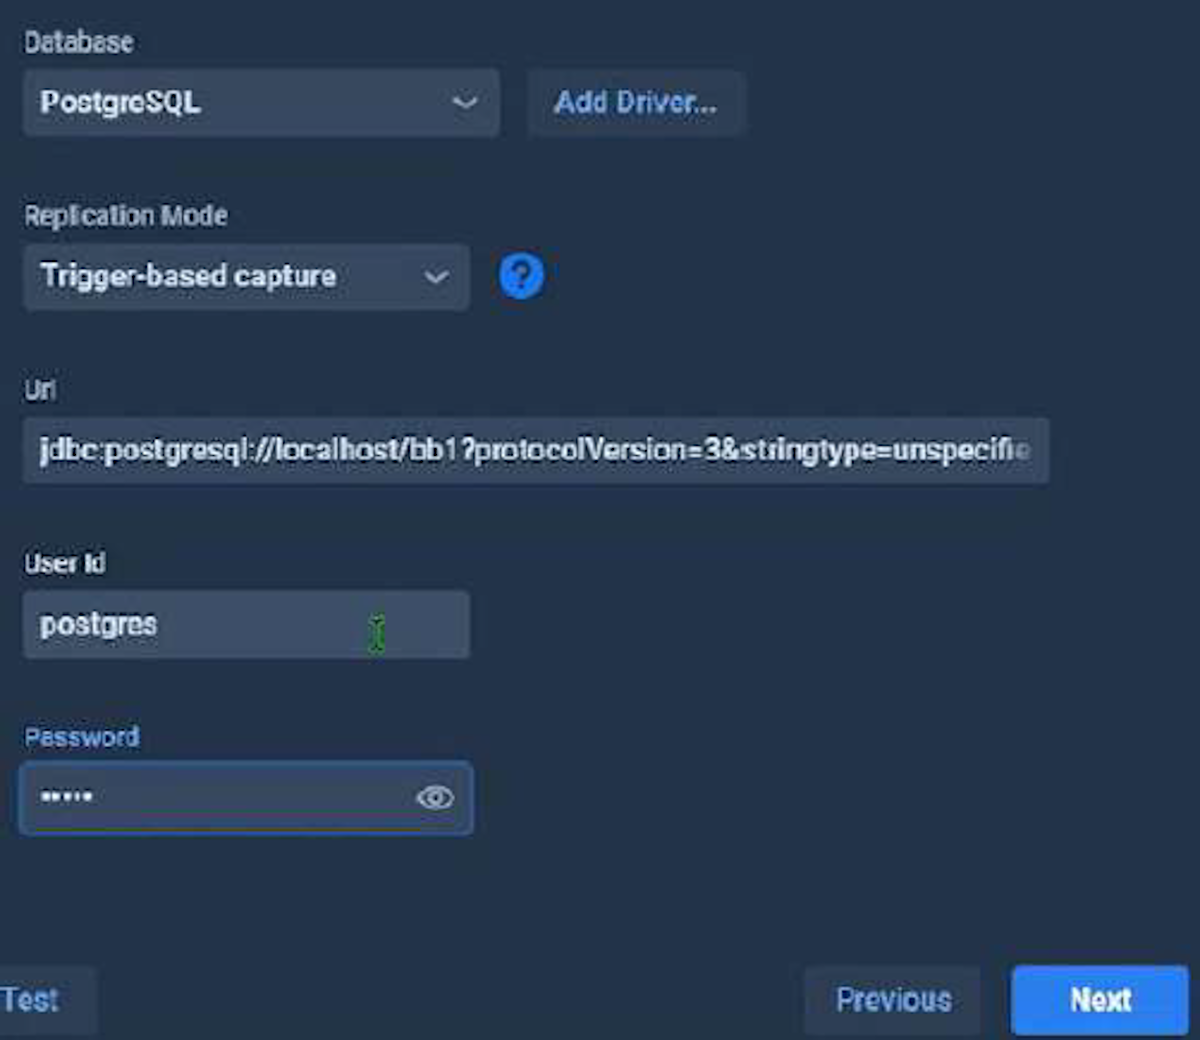
\includegraphics[width=0.5\textwidth]{images/SymmetricDS6.png}
		\caption{Parámetros para la conexión a PostgreSQL.}
		\label{fig:SymmetricDS6}
	\end{figure}
	Si los datos son correctos, la siguiente ventana mostrará el status todo yes y un visto indicando que todo se dió satisfactoriamente, a lo que debemos dar en \textit{next}, o caso contrario corregir los errores cometidos.
	\item \textbf{Tipo de replicación.} En este momento, está listo para seleccionar como será la replicación, esta ocasión como se quiere que sea de manera bidireccional, seleccionamos a la opción de “Secundary” y
	damos clic a \textit{next}.
	\item \textbf{Tipo de nodo.} Ahora se debe crear un nuevo nodo. Este nodo debe ser creado como primario. Al dar \textit{next}
	\item \textbf{Nombre del nodo.} En este paso se le debe asignar un nombre al nodo que se está creando. No es un nombre en particular, en este caso se le ha asignado el nombre de \textit{ndpg4}. Una vez asignado el nombre se da clic en \textit{next}.
	\item \textbf{Clave de la licencia.} En este momento se ingresa la licencia que debe haber llegado al correo
	electrónico, que generalmente es en un archivo de texto. El asistente muestra dos ocpiones para proporcionar la licencia como se muestra en la figura \ref{fig:SymmetricDS7}.
	
	\begin{figure}[hbt!]
		\centering
		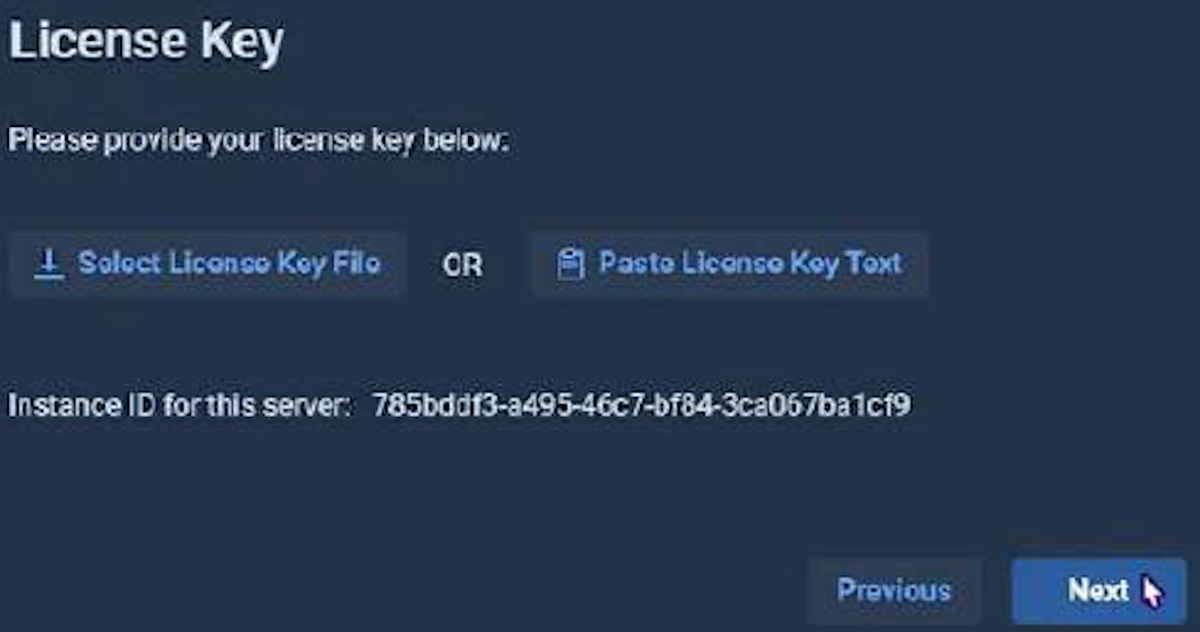
\includegraphics[width=0.5\textwidth]{images/SymmetricDS7.png}
		\caption{Proporcionar la licencia de SymmetricDS.}
		\label{fig:SymmetricDS7}
	\end{figure}
	\item \textbf{Credenciales para acceso al nodo.} Al dar clic en \textit{next}, nos mostrará la pantalla donde deberemos asignar una contraseña al user, que por defecto es admin, este nos permitirá acceder al nodo (desde consola).
	El asistente permite conocer la fortaleza de las credenciales que se está configurando, somo se muestra en la figura \ref{fig:SymmetricDS8}.
	\begin{figure}[hbt!]
		\centering
		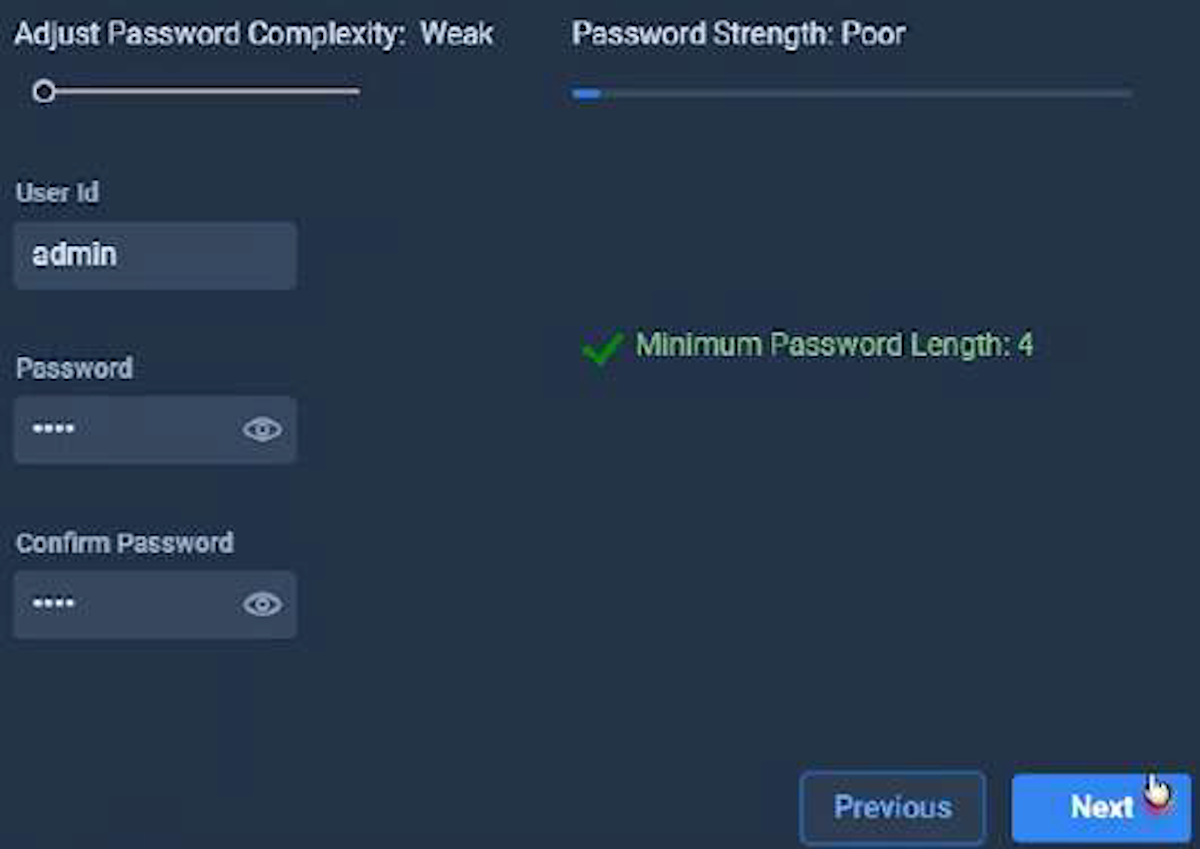
\includegraphics[width=0.5\textwidth]{images/SymmetricDS8.png}
		\caption{Credenciales de acceso al nodo.}
		\label{fig:SymmetricDS8}
	\end{figure}
	\item \textbf{Fin.} Al dar clic en \textit{next}, el asistente ha terminado de solicitar los datos para la instalación de SymmetricDS.
\end{itemize}
Una vez instalado el nodo, solicitará que se inicie sesión con las credenciales que se especificaron anteriormente (ver figura \ref{fig:SymmetricDS9}).

\begin{figure}[hbt!]
	\centering
	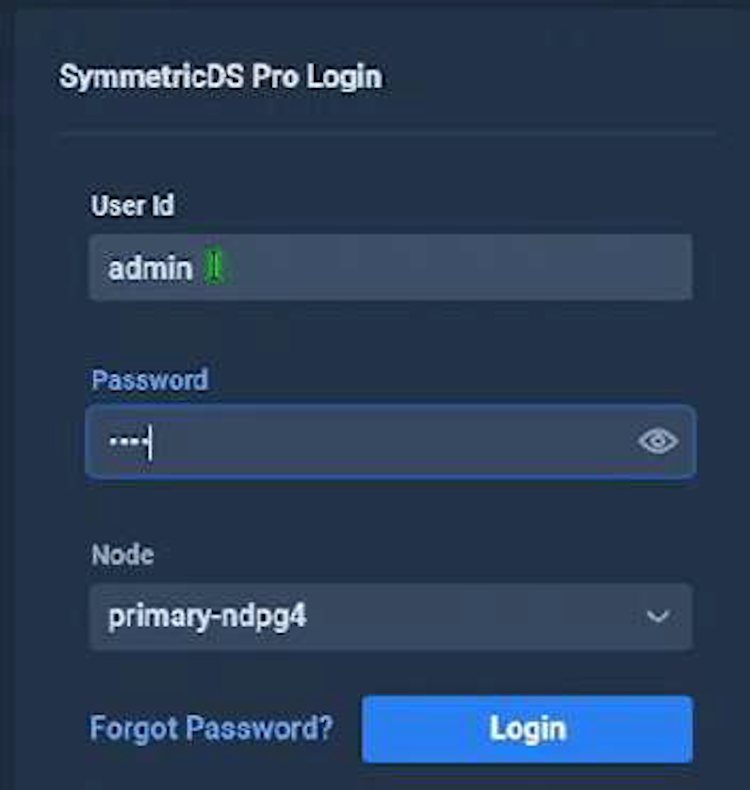
\includegraphics[width=0.35\textwidth]{images/SymmetricDS9.png}
	\caption{Inicio de sesión.}
	\label{fig:SymmetricDS9}
\end{figure}
Una vez que se inicia sesión, la misma aplicación mostrará que no existe una base de datos secundaria. Por lo tanto, se debe agregar una. En este caso se ha planeado trabajar con SQL Server. Se inicia su configuración dando clic en \textit{next}.

La configuración del nodo secundario, en este caso un servidor SQL Server, es muy similar a como se configuró en nodo primario o PostgreSQL (ver figura \ref{fig:SymmetricDS10}). Lo que se debe tener en cuenta que se seleccione el DBMS como SQL Server, la cadena de conexión, las credenciales de acceso (ver figure \ref{fig:SymmetricDS10a}), el tipo de nodo como nodo \textit{Secundary} (ver figura \ref{fig:SymmetricDS10b}), y finalmente está listo para configurar el nodo \ref{fig:SymmetricDS10c}.

\begin{figure}[htb!]
	\centering
	\begin{subfigure}{0.32\textwidth}
		\centering
		
\includegraphics[height=1.45in]{SymmetricDS10a.png}
		\caption{Configurar SQL Server}
		\label{fig:SymmetricDS10a}
	\end{subfigure}
	\hfill
	\begin{subfigure}{0.32\textwidth}
		\centering
		
\includegraphics[height=1.45in]{SymmetricDS10b.png}
		\caption{Selección del tipo de nodo}
		\label{fig:SymmetricDS10b}
	\end{subfigure}
	\hfill
	\begin{subfigure}{0.32\textwidth}
		\centering
		
\includegraphics[height=1.45in]{SymmetricDS10c.png}
		\caption{Todo listo para instalar}
		\label{fig:SymmetricDS10c}
	\end{subfigure}
	
	\caption{Configuración de SQL Server como nodo secundario}
	\label{fig:SymmetricDS10}
\end{figure}

En el caso que se está ilustrando, el asistente informa al usuario que no ha configurado ninguna tabla para la replicación, mostrando el número de tablas existentes en las bases de datos en los dos DBMS configurados (primario y secundario). En el siguiente paso aún no se seleccionará la(s) tabla(s) con la(s) que se va a trabajar. Sin embargo, el asistente permitirá seleccionare la dirección de la replicación, es decir de nodo principal a secundario, o de secundario a principal como se muestra en la figura \ref{fig:SymmetricDS11a}. Dando clic en \textit{next}, entonces el asistente le mostrará la interfaz de la figura \ref{fig:SymmetricDS11b} para que el usuario seleccione las diferentes tablas para la replicación de datos.

\begin{figure}[htb!]
	\centering
	\begin{subfigure}{0.48\textwidth}
		
\includegraphics[height=1.5in]{SymmetricDS11a.png}
		\caption{Dirección de la replicación}
		\label{fig:SymmetricDS11a}
	\end{subfigure}
	\hfill
	\begin{subfigure}{0.48\textwidth}
		
\includegraphics[height=1.5in]{SymmetricDS11b.png}
		\caption{Selección del tipo de nodo}
		\label{fig:SymmetricDS11b}
	\end{subfigure}
	\hfill
	\caption{Selección de las tablas}
	\label{fig:SymmetricDS11}
\end{figure}

Ahora bien, el asistente permitirá seleccionar la(s) base(s) de datos que recibirá(n) los datos (ver \ref{fig:SymmetricDS12}). Primero el asistente preguntará la dirección de la replicación, en una dirección o en ambas direcciones como se muestra en la figura \ref{fig:SymmetricDS12a}, para el caso práctico que se intenta ilustrar se seleccionará bidireccional. El siguiente paso cuya interfaz se muestra en la figura \ref{fig:SymmetricDS12b}, que sirve para seleccionar los nodos y bases de datos que recibirán los datos replicados.

\begin{figure}[htb!]
	\centering
	\begin{subfigure}{0.35\textwidth}
		\centering
		
\includegraphics[height=1.65in]{SymmetricDS12a.png}
		\caption{Dirección de la replicación}
		\label{fig:SymmetricDS12a}
	\end{subfigure}
	\hfill
	\begin{subfigure}{0.63\textwidth}
		\centering
		
\includegraphics[height=1.65in]{SymmetricDS12b.png}
		\caption{Selección del tipo de nodo}
		\label{fig:SymmetricDS12b}
	\end{subfigure}
	\hfill
	\caption{Selección de las bases de datos de los nodos}
	\label{fig:SymmetricDS12}
\end{figure}

Una vez que se han configurado todos los parámetros de la replicación de datos, se procede a realizar las acciones que se ejecutarán inicialmente en la réplica de datos. En la figura \ref{fig:SymmetricDS13a} muestra la interfaz para seleccionar el criterio para la carga de datos de está replicación. Entre esas acciones se pueden establecer: Que tablas se cargarán (todas, especificar ciertas tablas, o según el canal). Mientras que en la figura \ref{fig:SymmetricDS13b} muestra un resumen de la carga de datos que se va a realizar.

\begin{figure}[htb!]
	\centering
	\begin{subfigure}{0.48\textwidth}
		\centering
		
\includegraphics[height=2in]{SymmetricDS13a.png}
		\caption{Resumen de acciones de carga}
		\label{fig:SymmetricDS13a}
	\end{subfigure}
	\hfill
	\begin{subfigure}{0.48\textwidth}
		\centering
		
\includegraphics[height=2in]{SymmetricDS13b.png}
		\caption{Resumen de carga de datos}
		\label{fig:SymmetricDS13b}
	\end{subfigure}
	\hfill
	\caption{Carga de inicial de datos}
	\label{fig:SymmetricDS13}
\end{figure}
\noindent
Los resultados de la carga se muestran en la figura \ref{fig:SymmetricDS14}.

\begin{figure}[htb!]
	\centering
	
\includegraphics[width=\textwidth]{SymmetricDS14.png}
	\caption{Resultados de la carga inicial de datos}
	\label{fig:SymmetricDS14}
\end{figure}

A continuación se muestra como los datos se actualizan tanto en SQL Server como en PostgreSQL. Primero desde SQL Server se va a insertar 3 registros en la tabla de ciudades (ver listado \ref{lst:InsertInto}).

\begin{lstlisting}[language=SQL, caption={Insertar varias ciudades} \label{lst:InsertInto}]
INSERT INTO ciudades (nombre)
	VALUES ('Quito'),
	('Guayaquil'),
	('El Empalme');
\end{lstlisting}

Ahora se insertarán tres ciudades más en la misma tabla, así mismo desde SQL Server (ver listado \ref{lst:InsertIntoMas}).

\begin{lstlisting}[language=SQL, caption={Insertar múltiples ciudades}\label{lst:InsertIntoMas}]
INSERT INTO ciudades (nombre)
	VALUES ('Quioto'),
	('Guajayaquil'),
	('El Empallme');
\end{lstlisting}

\noindent
En la figura \ref{fig:SymmetricDS15} se muestra los dos momentos de la inserción de datos. Es decir después de la ejecución de las dos sentencias.

\begin{figure}[htb!]
	\centering
	\begin{subfigure}{0.48\textwidth}
		\centering
		
\includegraphics[height=2in]{SymmetricDS15a.png}
		\caption{Al insertar los 3 registros.}
		\label{fig:SymmetricDS15a}
	\end{subfigure}
	\hfill
	\begin{subfigure}{0.48\textwidth}
		\centering
		
\includegraphics[height=2in]{SymmetricDS15b.png}
		\caption{Al insertar los otros 3 registros.}
		\label{fig:SymmetricDS15b}
	\end{subfigure}
	\hfill
	\caption{Resultados al Insertar datos desde SQL Server}
	\label{fig:SymmetricDS15}
\end{figure}
Si todo se realizó de manera correcta, en la pestaña del Dashboard en la consola se mostrará una pantalla como en la figure \ref{fig:SymmetricDS16}. En la cual se muestra la información de las estadísticas sobre la ejecución de los procesos (inserciones). Se debe considerar que, este proceso puede llegar a tardar algún tiempo según la cantidad de información que se ingrese.

\begin{figure}[htb!]
	\centering
	
\includegraphics[width=\textwidth]{SymmetricDS16.png}
	\caption{Dashboard con la información de las estadísticas sobre la ejecución de los procesos}
	\label{fig:SymmetricDS16}
\end{figure}

Estos datos por ser replicación bidireccional, los mismos estarán en la base de datos de PostgreSQL, y si actualizamos la tabla, los datos que se ingresaron en SQL Server se ven reflejados como se muestra en la figura \ref{fig:SymmetricDS17}

\begin{figure}[htb!]
	\centering
	
\includegraphics[width=\textwidth]{SymmetricDS17.png}
	\caption{Datos en la tabla}
	\label{fig:SymmetricDS17}
\end{figure}

Ahora se procede a realizar las inserciones desde PostGreSQL, para comprobar la bidireccionalidad.

\begin{lstlisting}[language=SQL, caption={Insertar ciudades con nombres que contienen números}]
INSERT INTO ciudades (nombre)
	VALUES ('11Quito'),
	('1Guayaquil'),
	('E1l Empalme');
\end{lstlisting}

Ahora al abrir el Dashboard en la consola web se puede observar en la figura \ref{fig:SymmetricDS18} como esta cargando.

\begin{figure}[htb!]
	\centering
	
\includegraphics[width=\textwidth]{SymmetricDS18.png}
	\caption{Dashboard visualizando él éxito de las transacciones.}
	\label{fig:SymmetricDS18}
\end{figure}

Y en la captura de pantalla de la figura \ref{fig:SymmetricDS19} se muestran los datos en la tabla de la base de datos de SQL Server.

\begin{figure}[htb!]
	\centering
	
\includegraphics[width=\textwidth]{SymmetricDS19.png}
	\caption{Captura de pantalla de SQL Server con los datos actualizados.}
	\label{fig:SymmetricDS19}
\end{figure}


\subsubsection{Tolerancia a Fallos}
\noindent
En caso de un fallo en uno de los nodos de datos debido a un problema de hardware, una interrupción de red o cualquier otro motivo, el sistema sigue siendo operativo. Esto se debe a que los otros dos nodos de datos continúan funcionando y atendiendo las solicitudes de los usuarios. La tolerancia a fallos garantiza que el sistema no se vea afectado por un único punto de falla.

Además, se implementa un mecanismo de detección de fallos y conmutación por error. Si un nodo de datos se vuelve inaccesible, el sistema automáticamente redirige las solicitudes al nodo de datos más cercano disponible y actualiza la réplica del nodo fallido tan pronto como se restablezca la conectividad. Esto asegura la continuidad del servicio incluso en situaciones de fallos imprevistos.

Por lo tanto, la replicación de datos y la tolerancia a fallos en este ejemplo de base de datos distribuida garantizan que el sistema de reservas de vuelos en línea sea altamente disponible y resistente a problemas potenciales, brindando a los usuarios una experiencia confiable y sin interrupciones.

La tolerancia a fallos en los sistemas de gestión de bases de datos (DBMS) no es una propiedad intrínseca, sino más bien una característica que debe implementarse de manera consciente y específica en la arquitectura y configuración del sistema. La implementación de la tolerancia a fallos implica tomar medidas y adoptar estrategias para garantizar que el DBMS pueda continuar funcionando de manera efectiva incluso en presencia de fallos o errores inesperados.

Algunos DBMS ofrecen características y herramientas que facilitan la implementación de la tolerancia a fallos, pero aún así, es responsabilidad del administrador del sistema configurar y administrar estas características de manera adecuada. Algunas de las técnicas y características comunes utilizadas para lograr la tolerancia a fallos en sistemas de bases de datos incluyen:

\begin{enumerate}
	\item \textbf{Replicación de Datos:} Mantener copias redundantes de los datos en múltiples ubicaciones o nodos para que, en caso de fallo en un nodo, los datos estén disponibles en otros nodos.
	\item \textbf{Clustering y Alta Disponibilidad:} Utilizar configuraciones de clústeres y servidores redundantes para garantizar la disponibilidad continua del servicio en caso de fallo de hardware o software.
	\item \textbf{Copia de Seguridad y Recuperación:} Realizar copias de seguridad periódicas de los datos y tener procedimientos de recuperación en caso de pérdida de datos o fallo del sistema.
	\item \textbf{Detección de Fallos y Conmutación por Error:} Implementar sistemas de detección de fallos que alerten sobre problemas y permitan la conmutación automática a un sistema de respaldo en caso de fallo.
	\item \textbf{Tolerancia a Fallos de Red:} Considerar la redundancia de red y las rutas alternativas para garantizar la conectividad en caso de problemas de red.
	\item \textbf{Monitoreo Continuo:} Establecer sistemas de monitoreo y alerta para detectar y responder rápidamente a problemas antes de que afecten gravemente la operación.
	\item \textbf{Planificación de Capacidad:} Evitar la sobrecarga del sistema y garantizar que haya recursos suficientes disponibles para manejar situaciones de carga inesperadas.
\end{enumerate}
\begin{tcolorbox}[colback=yellow!10!white, colframe=blue!50!black, title=Resumiendo, coltitle=white]
	La tolerancia a fallos es una preocupación fundamental en la administración de bases de datos distribuidas y sistemas de gestión de bases de datos en general. Aunque algunos DBMS pueden ofrecer características específicas para facilitar la tolerancia a fallos, su implementación y gestión efectivas requieren la planificación y la adopción de estrategias adecuadas por parte de los administradores de sistemas y bases de datos.
\end{tcolorbox}

\subsection{Fragmentación}
\noindent
La fragmentación es el proceso de dividir una base de datos en fragmentos o particiones más pequeñas que se almacenan en diferentes nodos. Cada fragmento contiene un subconjunto de los datos totales y la fragmentación puede ser horizontal (por filas) o vertical (por columnas) dependiendo de cómo se dividan los datos.
\begin{itemize}
	\item \textbf{Fragmentación horizontal:} La fragmentación horizontal es un enfoque de fragmentación en el cual las filas de una tabla se dividen y distribuyen en diferentes nodos. Cada nodo contendrá un subconjunto de filas, lo que permite una distribución equilibrada de los datos.
	\item \textbf{Fragmentación vertical:} La fragmentación vertical es un enfoque de fragmentación en el cual las columnas de una tabla se dividen y distribuyen en diferentes nodos. Cada nodo contendrá un subconjunto de columnas, lo que permite una distribución eficiente de los datos según las necesidades de acceso y rendimiento.
\end{itemize}

\subsubsection{Fragmentación Vertical en PostgreSQL:}
\noindent
La fragmentación vertical implica dividir una tabla en columnas, de modo que cada fragmento contenga un subconjunto diferente de columnas. Esto es útil cuando se desea distribuir las columnas de una tabla en diferentes nodos o servidores según sus necesidades. Aquí hay un ejemplo:

Si se estuviese gestionando una base de datos distribuida para una empresa de comercio electrónico que vende productos en línea. Se tiene una tabla llamada "Productos" que contiene información sobre los productos, incluyendo detalles como el nombre, la descripción, el precio y la disponibilidad. Sin embargo, en algunos nodos de nuestra base de datos distribuida, sólo se necesita información sobre el nombre y la descripción de los productos, mientras que en otros nodos se necesita toda la información.

Se podría crear dos fragmentos de la tabla "Productos" de la siguiente manera:

Fragmento 1 (contiene solo el nombre y la descripción - listado \ref{lst:CreateSelect}). 

\begin{lstlisting}[language=SQL, caption={Crear una nueva tabla a partir de otra}\label{lst:CreateSelect}]
CREATE TABLE fragmento_productos_1 AS
	SELECT nombre, descripcion
	FROM productos;
\end{lstlisting}

Fragmento 2 (contiene todos los detalles del producto - listado \ref{lst:CreateCopyTable}).

\begin{lstlisting}[language=SQL, caption={Crear una tabla copia de productos} \label{lst:CreateCopyTable}]
CREATE TABLE fragmento_productos_2 AS
	SELECT *
	FROM productos;
\end{lstlisting}

De esta manera, los nodos que solo necesitan el nombre y la descripción de los productos pueden acceder al Fragmento 1, mientras que aquellos que requieren todos los detalles pueden acceder al Fragmento 2. Esto permite una distribución más eficiente de los datos según las necesidades de cada nodo.

\subsubsection{Fragmentación Horizontal en PostgreSQL}
\noindent
La fragmentación horizontal implica dividir una tabla en filas, de modo que cada fragmento contenga un subconjunto diferente de filas. Esto es útil cuando se desea distribuir datos de una tabla en función de un criterio específico. Aquí hay un ejemplo:

Como ejemplo se puede considerar que se está gestionando una base de datos distribuida para una cadena de tiendas minoristas en diferentes ubicaciones geográficas. Se tiene una tabla llamada "Ventas" que registra las ventas diarias en todas las tiendas. Para mejorar el rendimiento y facilitar el acceso a los datos, se decide fragmentar la tabla por ubicación geográfica.

Se podría crear fragmentos de la tabla "Ventas" de la siguiente manera:

Fragmento 1 (registros de ventas de Nueva York - listado \ref{lst:CreateTableNewYorkSales}).

\begin{lstlisting}[language=SQL, caption={Crear una tabla con ventas de Nueva York} \label{lst:CreateTableNewYorkSales}]
CREATE TABLE fragmento_ventas_ny AS
	SELECT *
	FROM ventas
	WHERE ubicacion = 'Nueva York';
\end{lstlisting}

\noindent
Fragmento 2 (registros de ventas de Los Ángeles - listado \ref{lst:CreateTableLosAngelesSales}).

\begin{lstlisting}[language=SQL, caption={Crear una tabla con ventas de Los Ángeles} \label{lst:CreateTableLosAngelesSales}]
CREATE TABLE fragmento_ventas_la AS
	SELECT *
	FROM ventas
	WHERE ubicacion = 'Los %Á%ngeles';
\end{lstlisting}

Fragmento 3 (registros de ventas de Chicago - listado \ref{lst:CreateTableChicagoSales}).

\begin{lstlisting}[language=SQL, caption={Crear una tabla con ventas de Chicago} \label{lst:CreateTableChicagoSales}]
CREATE TABLE fragmento_ventas_chicago AS
	SELECT *
	FROM ventas
	WHERE ubicacion = 'Chicago';
\end{lstlisting}

Cada fragmento contiene los registros de ventas correspondientes a una ubicación geográfica específica. Esto facilita la recuperación de datos de ventas para cada ubicación de manera eficiente y reduce la carga en los nodos de la base de datos distribuida.

\subsection{Consistencia y Coherencia de datos}
\noindent
La consistencia en una base de datos distribuida se refiere a la propiedad de que todos los nodos vean y operen con datos consistentes. Por su parte la coherencia en una base de datos distribuida se refiere a la propiedad de que todos los nodos vean una versión consistente de los datos en todo momento. Esto implica que los nodos reflejen las actualizaciones de manera ordenada y coherente para mantener la integridad de los datos.

\subsubsection{Consistencia y Coherencia de Datos en SQL Server}
\noindent
Se puede suponer que se está gestionando una base de datos distribuida para una cadena de tiendas minoristas en diferentes ubicaciones geográficas. Se tiene una tabla llamada "Inventario" que registra la cantidad de productos disponibles en cada tienda. Para garantizar la consistencia y la coherencia de datos, se requiere asegurar de que las siguientes condiciones se cumplan en todo momento:

\begin{itemize}
	\item La cantidad de productos en el inventario nunca sea negativa.
	\item Cuando se realiza una venta en una tienda, la cantidad de productos disponibles se actualice correctamente.
	\item Los cambios en el inventario se reflejen en todas las ubicaciones de manera consistente y en tiempo real.
\end{itemize}
Para lograr esto, puedes utilizar las siguientes estrategias y sentencias SQL en SQL Server:

\begin{enumerate}
	\item \textbf{Utilizar Restricciones de Integridad.} Se puede definir restricciones de integridad para garantizar que la cantidad de productos nunca sea negativa. Por ejemplo en el listado de código \ref{lst:CreateTable}:
	
	\begin{lstlisting}[language=SQL, caption={Crear tabla Inventario con restricción CHECK} \label{lst:CreateTable}]
CREATE TABLE Inventario (
	ProductoID INT PRIMARY KEY,
	Cantidad INT CHECK (Cantidad >= 0),
	Ubicacion VARCHAR(50)
);
	\end{lstlisting}
	
	La restricción CHECK (ver ejemplo \ref{lst:CreateTable}) asegura que la cantidad no sea negativa en ningún momento.
	\item \textbf{Transacciones para Actualizar el Inventario.} Cuando se realiza una venta en una tienda, se debe asegurar de que la cantidad de productos disponibles se actualice correctamente. Se puede hacer esto utilizando transacciones en SQL Server para garantizar que las operaciones sean atómicas y consistentes. Por ejemplo (\label{eje:ConCohe}):
	
	\texttt{\\BEGIN TRANSACTION;\\
		-- Restar la cantidad vendida del inventario\\
		UPDATE Inventario\\
		SET Cantidad = Cantidad - @CantidadVendida\\
		WHERE ProductoID = @ProductoID AND Ubicacion = @Ubicacion;\\ \\
		-- Registrar la venta en la tabla de ventas\\
		INSERT INTO Ventas (ProductoID, CantidadVendida, Fecha, Ubicacion) \\
		VALUES (@ProductoID, @CantidadVendida, GETDATE(), @Ubicacion);\\ \\
		COMMIT;
	}
	\item \textbf{Uso de Replicación o Distribución de Datos.} Para asegurarte de que los cambios en el inventario se reflejen en todas las ubicaciones de manera consistente y en tiempo real, puedes utilizar características de replicación o distribución de datos en SQL Server. Esto garantiza que los datos estén sincronizados en todas las ubicaciones, lo que mejora la coherencia de datos en todo el sistema.
\end{enumerate}
Estas estrategias y sentencias SQL en SQL Server son ejemplos de cómo puedes garantizar la consistencia y la coherencia de datos en una base de datos distribuida. Mantener un control estricto sobre las operaciones de actualización y utilizar restricciones de integridad son prácticas clave para mantener datos confiables y coherentes en entornos distribuidos.

\subsection{Atomicidad}
\noindent
La atomicidad se refiere a la propiedad de una operación en una base de datos distribuida de ser una unidad atómica e indivisible. Esto significa que una operación se realiza en su totalidad o no se realiza en absoluto, evitando así resultados parciales o inconsistentes (ver ejemplo \ref{eje:ConCohe}).

\subsection{Consenso}
\noindent
El consenso es un proceso en el cual los nodos de una base de datos distribuida llegan a un acuerdo sobre una decisión o valor común. Esto se logra mediante algoritmos de consenso, como el algoritmo de consenso de Paxos o el algoritmo de tolerancia a fallas bizantinas (BFT), que permiten a los nodos llegar a un consenso incluso si algunos nodos fallan o son maliciosos.

El "\textit{consenso}" en el contexto de las bases de datos distribuidas se refiere a la necesidad de garantizar que todas las réplicas de datos en diferentes nodos estén sincronizadas y reflejen la misma información, incluso en presencia de operaciones concurrentes y actualizaciones. Una técnica común para lograr el consenso es la utilización de transacciones distribuidas. A continuación, se presenta el ejemplo \ref{eje:consenso} de cómo se puede implementar el consenso con SQL Server mediante el uso de transacciones distribuidas.

Si se está gestionando una base de datos distribuida para una cadena de tiendas minoristas en diferentes ubicaciones geográficas, entonces, se desea garantizar que las ventas realizadas en cada tienda se registren de manera coherente y que los totales de ventas se actualicen correctamente en tiempo real en una base de datos centralizada. En este escenario, se puede utilizar transacciones distribuidas para lograr el consenso.

\subsubsection{Consenso con Transacciones Distribuidas en SQL Server}
\noindent
\begin{enumerate}
	\item Se tiene una base de datos centralizada llamada "VentasCentrales" que almacena los totales de ventas consolidados de todas las tiendas.
	\item Cada tienda tiene su propia base de datos local llamada "VentasTiendaX" donde registra las ventas realizadas en esa ubicación.
	\item Para garantizar el consenso y mantener los totales de ventas actualizados en la base de datos central, se puede utilizar transacciones distribuidas. Se debe asegurar que todas las bases de datos estén configuradas para admitir transacciones distribuidas.
	\item Cuando se realiza una venta en una tienda local, se inicia una transacción distribuida que abarca tanto la base de datos local como la base de datos central. Por ejemplo \label{eje:consenso}:
	
	\texttt{\\BEGIN DISTRIBUTED TRANSACTION;\\
		-- Actualizar la base de datos local de la tienda\\
		INSERT INTO VentasTiendaX (ProductoID, CantidadVendida, Fecha)\\
		VALUES (@ProductoID, @CantidadVendida, GETDATE());\\ \\
		-- Actualizar la base de datos centralizada\\
		UPDATE VentasCentrales\\
		SET TotalVentas = TotalVentas + @CantidadVendida\\
		WHERE Tienda = 'TiendaX';\\ \\
		COMMIT;\\
	}
	\item Si la transacción se completa con éxito en ambas bases de datos (local y central), se garantiza que los totales de ventas reflejen correctamente la última venta realizada en esa tienda y que haya coherencia entre todas las ubicaciones.
\end{enumerate}
Con este ejemplo se trata de ilustrar cómo se puede implementar el consenso utilizando transacciones distribuidas en SQL Server. Las transacciones distribuidas garantizan que todas las operaciones relacionadas con una venta se completen de manera exitosa o se reviertan de manera coherente en todas las bases de datos involucradas, asegurando así que los datos se mantengan consistentes en todo el sistema distribuido.

\subsection{Escalabilidad}
\noindent
La escalabilidad se refiere a la capacidad de una base de datos distribuida para manejar un aumento en la carga de trabajo y el tamaño de los datos. Una base de datos distribuida escalable puede agregar nuevos nodos y distribuir la carga de trabajo de manera eficiente para mantener un rendimiento óptimo.

En las bases de datos distribuidas, es común hablar de escalabilidad tanto horizontal como vertical. Ambos conceptos se refieren a diferentes enfoques para aumentar la capacidad de almacenamiento y procesamiento de datos en un entorno distribuido.

\begin{itemize}
	\item \textbf{Escalabilidad horizontal (también conocida como escalabilidad "scale-out"):} Se refiere a la capacidad de una base de datos distribuida para manejar un mayor volumen de datos y carga de trabajo al agregar más nodos al sistema. En este enfoque, se distribuyen los datos entre múltiples nodos, lo que permite un crecimiento horizontal del sistema. Cada nodo tiene una fracción de los datos y puede manejar parte de la carga de trabajo. La escalabilidad horizontal se logra agregando nuevos nodos al clúster y distribuyendo los datos y las tareas entre ellos. Este enfoque ofrece una mayor capacidad de procesamiento y almacenamiento a medida que se agregan más nodos al sistema.
	\item \textbf{Escalabilidad vertical (también conocida como escalabilidad "scale-up"):} Se refiere a la capacidad de una base de datos distribuida para manejar un mayor volumen de datos y carga de trabajo al aumentar los recursos de hardware en un nodo existente. En lugar de agregar más nodos, se mejoran las capacidades de procesamiento, almacenamiento y memoria de un único nodo. Esto implica la actualización de los componentes físicos del hardware, como el procesador, la memoria RAM o el disco duro. La escalabilidad vertical permite un aumento en la capacidad de procesamiento y almacenamiento en un solo nodo, pero tiene un límite físico en términos de cuántos recursos se pueden agregar.
\end{itemize}

\begin{tcolorbox}[colback=yellow!10!white, colframe=blue!50!black, title=Resumiendo, coltitle=white]
	La escalabilidad horizontal se basa en la adición de más nodos para distribuir la carga y los datos, mientras que la escalabilidad vertical se basa en mejorar los recursos de hardware en un nodo existente. Ambos enfoques tienen sus ventajas y limitaciones, y la elección depende de los requisitos y características específicas de la base de datos distribuida.
\end{tcolorbox}

\section{Definición de base de datos distribuida}
\noindent
Una base de datos distribuida es un sistema de gestión de bases de datos (SGBD) en el cual los datos se almacenan y se gestionan en múltiples nodos o servidores interconectados en una red. Cada nodo contiene una parte de los datos y puede procesar consultas y realizar operaciones en su propio conjunto de datos local. Los nodos se comunican entre sí para compartir y sincronizar datos, lo que permite la distribución y el acceso eficiente a los datos en entornos distribuidos.

\subsection{Características}
\noindent
las características de las bases de datos distribuidas destacan los aspectos fundamentales que hacen que las bases de datos distribuidas sean una solución eficiente y confiable para satisfacer las necesidades de almacenamiento y gestión de datos en entornos complejos. Estas características clave incluyen:

\begin{itemize}
	\item \textbf{Distribución:} Los datos se almacenan y se distribuyen en múltiples nodos, lo que mejora la disponibilidad, la escalabilidad y la tolerancia a fallos.
	\item \textbf{Replicación:} Los datos se pueden replicar en varios nodos para mejorar la disponibilidad y la redundancia.
	\item \textbf{Coordinación y sincronización:} Los nodos se comunican y se sincronizan para garantizar la coherencia y la integridad de los datos distribuidos.
	\item \textbf{Transparencia:} Los usuarios y las aplicaciones pueden interactuar con la base de datos distribuida como si fuera una base de datos centralizada, sin conocer los detalles de la distribución física de los datos.
\end{itemize}
Estas características combinadas forman la columna vertebral de nuestra solución de base de datos distribuida, brindando un rendimiento excepcional, confiabilidad y facilidad de uso para satisfacer las demandas de los entornos modernos de gestión de datos.

\subsection{Especificaciones de uso}
\noindent
\begin{itemize}
	\item \textbf{Arquitectura cliente-servidor:} Los clientes se conectan a los nodos servidores para realizar operaciones y acceder a los datos distribuidos.
	\item \textbf{Protocolos de comunicación:} Se utilizan protocolos como TCP/IP, HTTP o mensajes en cola para facilitar la comunicación entre los nodos.
	\item \textbf{Optimización de consultas:} Se emplean técnicas de optimización para mejorar el rendimiento y la eficiencia en la ejecución de consultas distribuidas.
	\item \textbf{Seguridad y control de acceso:} Se implementan mecanismos de seguridad para proteger los datos y controlar el acceso a ellos en un entorno distribuido.
\end{itemize}

\subsection{Aplicaciones}
\noindent
\begin{itemize}
	\item \textbf{Aplicaciones empresariales:} Las bases de datos distribuidas se utilizan en entornos empresariales para gestionar datos a gran escala en múltiples ubicaciones geográficas.
	\item \textbf{Sistemas de seguimiento y logística:} Permiten el seguimiento y la gestión de inventarios, envíos y rutas en tiempo real en entornos distribuidos.
	\item \textbf{Redes sociales y aplicaciones web:} Las bases de datos distribuidas son fundamentales para gestionar grandes volúmenes de datos generados por usuarios y proporcionar respuestas rápidas a las consultas.
	\item \textbf{Aplicaciones científicas y de investigación:} Permiten el procesamiento y análisis distribuido de grandes conjuntos de datos para investigaciones científicas, análisis de datos y simulaciones.
\end{itemize}

\subsection{Ejemplos}
\noindent
\begin{itemize}
	\item \textit{Google Spanner:} Un sistema de bases de datos distribuidas desarrollado por Google que ofrece una alta disponibilidad, escalabilidad y consistencia global de los datos.
	\item \textit{Apache Cassandra:} Una base de datos distribuida escalable y de alto rendimiento utilizada por grandes empresas como Facebook y Netflix para gestionar grandes cantidades de datos en múltiples ubicaciones.
	\item \textit{Amazon DynamoDB:} Un servicio de bases de datos distribuidas completamente administrado que ofrece almacenamiento escalable y rendimiento rápido para aplicaciones en la nube.
	\item \textit{MongoDB:} Una base de datos NoSQL distribuida que permite el almacenamiento y procesamiento distribuido de datos no estructurados en múltiples nodos.
\end{itemize}
Estos ejemplos ilustran cómo las bases de datos distribuidas se utilizan en diversos escenarios para satisfacer las necesidades de almacenamiento y procesamiento de datos en entornos distribuidos.

\section{Arquitecturas de Bases de Datos}
\noindent
Las bases de datos pueden tener diferentes arquitecturas según cómo se estructuran y almacenan los datos. Algunas arquitecturas comunes son:

\subsection{Arquitectura de Base de Datos Centralizada}
\noindent
En esta arquitectura, todos los datos se almacenan en un único servidor centralizado. Las aplicaciones y usuarios acceden a los datos a través de este servidor. Es una arquitectura sencilla pero puede tener limitaciones en términos de escalabilidad y disponibilidad. Un ejemplo podría ser una base de datos centralizada utilizada por una pequeña empresa para gestionar su inventario y registros de clientes en una sola ubicación.

Para implementar una base de datos centralizada, se puede utilizar sistemas de gestión de bases de datos tradicionales como MySQL, PostgreSQL o Microsoft SQL Server. Se debe asegurar de que el servidor sea escalable y pueda manejar las necesidades de almacenamiento y rendimiento de la empresa en cuestión.

\subsection{Arquitectura Cliente-Servidor}
\noindent
En esta arquitectura, los datos se almacenan en un servidor central, y los clientes se conectan a este servidor para acceder y manipular los datos. El servidor es responsable de gestionar las solicitudes de los clientes y realizar operaciones en la base de datos. Es una arquitectura comúnmente utilizada en entornos empresariales.

Un ejemplo podría ser una base de datos de comercio electrónico en la que los clientes (aplicaciones web o móviles) se conectan a servidores que almacenan información de productos, pedidos y usuarios.

Por ejemplo, en una base de datos distribuida de comercio electrónico cliente-servidor:
\begin{itemize}
	\item Los servidores de aplicaciones manejan la lógica de la aplicación y se conectan a los servidores de bases de datos para recuperar información de productos.
	\item Los servidores de bases de datos pueden estar distribuidos geográficamente para mejorar el rendimiento y la disponibilidad.
\end{itemize}

\subsection{Arquitectura de Base de Datos Distribuida}
\noindent
En esta arquitectura, los datos se distribuyen en múltiples servidores interconectados, también conocidos como nodos. Cada nodo puede contener una parte de los datos y tiene la capacidad de procesar consultas y realizar operaciones en su propio conjunto de datos local. Los nodos se comunican entre sí para compartir y sincronizar datos. Esta arquitectura ofrece ventajas como escalabilidad, disponibilidad y tolerancia a fallos.

En las bases de datos distribuidas, se puede hablar tanto de bases de datos homogéneas como de bases de datos heterogéneas, dependiendo de la uniformidad o diversidad de los sistemas de gestión de bases de datos (SGBD) utilizados en el entorno distribuido.

\begin{itemize}
	\item \textbf{Bases de datos homogéneas:} En una base de datos distribuida homogénea, todos los nodos o sistemas que componen la infraestructura utilizan el mismo sistema de gestión de bases de datos (SGBD) y siguen un modelo de datos coherente. Esto significa que todos los nodos almacenan y gestionan los datos de la misma manera, utilizando las mismas reglas de integridad, esquemas de almacenamiento y lenguajes de consulta. La ventaja de las bases de datos homogéneas es la simplicidad en el diseño y mantenimiento, ya que todos los nodos son interoperables y comparten una arquitectura común. Esto facilita la distribución de datos y consultas entre los nodos, así como la realización de operaciones de transacciones y mantenimiento de la consistencia global.
	\item \textbf{Bases de datos heterogéneas:} En una base de datos distribuida heterogénea, los nodos o sistemas que conforman la infraestructura utilizan diferentes sistemas de gestión de bases de datos (SGBD) y pueden seguir modelos de datos diferentes. Cada nodo puede tener su propio SGBD con su propio conjunto de reglas de integridad, esquemas de almacenamiento y lenguajes de consulta. Esto puede generar desafíos en términos de interoperabilidad y consistencia de datos, ya que los diferentes sistemas pueden tener diferentes formas de gestionar y representar la información. Para abordar la heterogeneidad, se pueden utilizar mecanismos de mediación y traducción de datos para permitir la comunicación y la integración de los diferentes sistemas. Las bases de datos heterogéneas ofrecen flexibilidad en términos de elección de sistemas y modelos de datos, pero también pueden requerir más esfuerzo en términos de diseño, implementación y mantenimiento debido a la diversidad de tecnologías involucradas.
\end{itemize}
Para implementar una base de datos distribuida homogénea, se puede configurar clusteres de bases de datos como \textit{Galera Cluster} para \textit{MySQL} o usar bases de datos en la nube como \textit{Amazon RDS}. Para una base de datos distribuida heterogénea, se debe utilizar herramientas de federación y replicación de datos que sean compatibles con los diferentes sistemas de gestión de bases de datos que se esté utilizando.

\begin{tcolorbox}[colback=yellow!10!white, colframe=blue!50!black, title=Resumiendo, coltitle=white]
	Las bases de datos distribuidas homogéneas utilizan un único sistema de gestión de bases de datos y un modelo de datos coherente en todos los nodos, mientras que las bases de datos distribuidas heterogéneas pueden tener diferentes sistemas de gestión de bases de datos y modelos de datos en cada nodo, lo que requiere mecanismos adicionales para garantizar la interoperabilidad y la consistencia de los datos.
\end{tcolorbox}

\subsection{Bases de Datos Distribuidas Federadas}
\noindent
En este tipo de arquitectura, múltiples bases de datos autónomas se unen y se presentan como una única base de datos lógica para los usuarios. Cada base de datos federada conserva su autonomía y se comunica con otras bases de datos según sea necesario.

Por ejemplo, en una base de datos federada de una empresa multinacional:
\begin{itemize}
	\item Cada sucursal de la empresa tiene su propia base de datos local con datos de empleados y operaciones locales.
	\item Una base de datos federada centraliza la información de todas las sucursales y permite a los usuarios acceder a los datos de todas las sucursales como si fueran una sola base de datos.
\end{itemize}

\subsection{Arquitectura de Base de Datos en Memoria (In-Memory)}
\noindent
En esta arquitectura, la base de datos almacena y gestiona los datos completamente en la memoria principal del servidor en lugar de en el almacenamiento en disco tradicional. Esto acelera significativamente el rendimiento de las consultas y transacciones. Un ejemplo podría ser una base de datos en memoria utilizada en una aplicación de comercio electrónico para gestionar el catálogo de productos y el carrito de compras en tiempo real.

Para implementar una base de datos en memoria, puedes utilizar sistemas como Redis, Memcached o SQL Server con tablas en memoria. Debes diseñar cuidadosamente la estructura de datos y asegurarte de que haya suficiente RAM disponible en el servidor para contener todos los datos necesarios.

\subsection{Arquitectura de Base de Datos Orientada a Columnas}
\noindent
En esta arquitectura, los datos se almacenan y se gestionan en columnas en lugar de filas, lo que es especialmente eficiente para operaciones analíticas y consultas que involucran solo un subconjunto de columnas. Un ejemplo podría ser una base de datos orientada a columnas utilizada en una empresa de análisis de datos para almacenar registros de registros de clics en un sitio web.

Su implementación se Puede llevar a cabo en  una base de datos orientada a columnas utilizando sistemas como \textit{Apache Cassandra} o \textit{Amazon Redshift}. Se debe diseñar el esquema de la base de datos de manera que las columnas sean optimizadas para tipos específicos de consultas y análisis.

Un ejemplo real de una base de datos orientada a columnas podría ser una base de datos utilizada por una empresa de análisis de datos para almacenar y analizar registros de clics de un sitio web. En este escenario, la empresa necesita gestionar grandes cantidades de datos de registro de clics de usuarios para comprender el comportamiento en el sitio web y tomar decisiones comerciales basadas en análisis.

\subsubsection{Implementación con Apache Cassandra}
\noindent
Al suponer que la empresa decide utilizar Apache Cassandra para implementar esta base de datos orientada a columnas. Cassandra es una base de datos distribuida y escalable que se adapta bien a cargas de trabajo de escritura intensiva y consultas de lectura de datos a gran escala. Aquí está cómo podría ser la implementación:

\begin{enumerate}
	\item \textbf{Diseño del Esquema de la Base de Datos.} En Cassandra, el diseño del esquema se basa en cómo se realizarán las consultas. Dado que la empresa desea realizar análisis sobre los registros de clics, el esquema se optimizará para tipos específicos de consultas. Por ejemplo, podría haber columnas para registrar el identificador de usuario, la URL visitada, la marca de tiempo del clic y otros atributos relevantes.
	\item \textbf{Modelo de Datos de Columnas.} En lugar de tener una fila por cada registro de clic, se crearán columnas para cada atributo de interés. Esto significa que cada fila en la base de datos tendrá múltiples columnas, cada una con un valor específico. Por ejemplo, podría haber una columna para el ID de usuario, otra para la URL y otra para la marca de tiempo.
	\item \textbf{Distribución de Datos.} Cassandra es una base de datos distribuida, por lo que los datos se distribuirán en múltiples nodos. Esto permite una escalabilidad horizontal y un alto rendimiento. Los registros de clics se distribuirán en función de alguna clave de partición, como el identificador de usuario o la URL visitada, para que los datos estén distribuidos de manera uniforme entre los nodos.
	\item \textbf{Almacenamiento y Consultas.} Cassandra almacena datos de manera eficiente en columnas y es capaz de manejar consultas analíticas a gran escala. La empresa puede ejecutar consultas para realizar análisis, como calcular estadísticas de clics, identificar patrones de comportamiento de usuarios o generar informes personalizados.
\end{enumerate}
En este ejemplo, una base de datos orientada a columnas como Apache Cassandra permite a la empresa de análisis de datos almacenar y consultar grandes volúmenes de registros de clics de manera eficiente, lo que les ayuda a obtener información valiosa sobre el comportamiento de los usuarios en el sitio web y a tomar decisiones informadas para mejorar la experiencia del usuario y el rendimiento del sitio.

\subsection{Arquitectura de bases de Datos Distribuidas Peer-to-Peer}
\noindent
En esta arquitectura, los nodos (peers) de la red son iguales y se comunican entre sí para compartir datos. Un ejemplo podría ser una red peer-to-peer de intercambio de archivos donde cada nodo almacena una parte de los archivos y los usuarios pueden descargar desde varios nodos al mismo tiempo.

Por ejemplo, en una red peer-to-peer de intercambio de archivos:

\begin{itemize}
	\item Cada usuario que comparte archivos tiene una copia local de los archivos y actúa como un nodo en la red.
	\item Cuando un usuario busca un archivo, su solicitud se propaga a través de la red y se descarga desde múltiples nodos que tienen el archivo.
\end{itemize}

\section{Tipos de Almacenamiento de bases de datos distribuidas}
\noindent
En las bases de datos distribuidas, existen diferentes tipos de almacenamiento que se utilizan para gestionar y almacenar los datos distribuidos de manera eficiente. A continuación, se describen los tipos de almacenamiento más comunes:

\subsection{Almacenamiento local}
\noindent
Cada nodo en una base de datos distribuida tiene su propio almacenamiento local donde almacena una parte de los datos. Cada nodo es responsable de administrar y mantener sus propios datos. Este enfoque permite una mayor independencia y autonomía en cada nodo, pero puede resultar en una mayor complejidad para mantener la coherencia y la sincronización de los datos entre los nodos.

\subsubsection{Características:}
\noindent
\begin{itemize}
	\item Cada nodo en la red tiene su propio almacenamiento local.
	\item Cada nodo es responsable de administrar y mantener sus propios datos.
	\item Permite una mayor independencia y autonomía en cada nodo.
\end{itemize}

\subsubsection{Ventajas:}
\noindent
\begin{itemize}
	\item Mayor control sobre los datos en cada nodo.
	\item Menor dependencia de la red y otros nodos.
\end{itemize}

\subsubsection{Desventajas:}
\noindent
\begin{itemize}
	\item Mayor complejidad para mantener la coherencia y la sincronización de los datos entre los nodos.
	\item Puede generar duplicación de datos si se necesita acceso a los mismos datos en múltiples nodos.
\end{itemize}

\subsubsection{Ejemplos de servidores de bases de datos habilitados para el almacenamiento local:}
\noindent
\begin{itemize}
	\item \textbf{SQLite:} Un servidor de base de datos ligero y sin servidor que permite el almacenamiento local y es ampliamente utilizado en aplicaciones móviles y embebidas.
	\item \textbf{MySQL:} Un popular servidor de bases de datos relacional que se puede configurar para operar en modo local.
\end{itemize}

\subsection{Almacenamiento distribuido}
\noindent
Los datos se distribuyen entre múltiples nodos en la red. Cada nodo almacena una parte de los datos, y los nodos se comunican y se sincronizan entre sí para compartir y acceder a los datos distribuidos. Este enfoque permite una mayor escalabilidad y rendimiento, ya que la carga de trabajo se distribuye entre varios nodos. Sin embargo, también puede requerir una mayor gestión y coordinación para garantizar la coherencia de los datos.

\subsubsection{Características:}
\noindent
\begin{itemize}
	\item Los datos se distribuyen entre múltiples nodos en la red.
	\item Cada nodo almacena una parte de los datos y se comunica con otros nodos para compartir y acceder a los datos.
\end{itemize}
\subsubsection{Ventajas:}
\begin{itemize}
	\item Mayor escalabilidad y rendimiento, ya que la carga de trabajo se distribuye entre varios nodos.
	\item Mayor tolerancia a fallos, ya que la pérdida de un nodo no afecta la disponibilidad de los datos.
\end{itemize}

\subsubsection{Desventajas:}
\noindent
\begin{itemize}
	\item Mayor complejidad para mantener la coherencia de los datos distribuidos.
	\item Requiere una gestión y coordinación efectivas para garantizar la sincronización de los datos entre los nodos.
\end{itemize}

\subsubsection{Ejemplos de servidores de bases de datos habilitados para el almacenamiento distribuido:}
\noindent
\begin{itemize}
	\item \textbf{Apache Cassandra:} Una base de datos distribuida y altamente escalable que proporciona replicación y particionamiento automático de datos.
	\item \textbf{Amazon DynamoDB:} Un servicio de base de datos NoSQL completamente administrado que ofrece almacenamiento y consulta distribuidos.
\end{itemize}

\subsection{Almacenamiento replicado}
\noindent
Los datos se replican en varios nodos en la red. Cada réplica contiene una copia idéntica de los datos y se mantiene actualizada mediante mecanismos de sincronización. La replicación mejora la disponibilidad y la tolerancia a fallos, ya que, si un nodo falla, los datos aún están disponibles en otras réplicas. Sin embargo, la replicación también puede aumentar la complejidad y el costo de almacenamiento.

\subsubsection{Características:}
\noindent
\begin{itemize}
	\item Los datos se replican en múltiples nodos en la red.
	\item Cada réplica contiene una copia idéntica de los datos y se mantiene actualizada mediante mecanismos de sincronización.
\end{itemize}

\subsubsection{Ventajas:}
\noindent
\begin{itemize}
	\item Mayor disponibilidad y tolerancia a fallos, ya que si un nodo falla, los datos aún están disponibles en otras réplicas.
	\item Mejor rendimiento y latencia, ya que los datos están distribuidos en ubicaciones geográficas cercanas.
\end{itemize}

\subsubsection{Desventajas:}
\noindent
\begin{itemize}
	\item Mayor complejidad y costo de almacenamiento debido a la duplicación de datos.
	\item Mayor sobrecarga en términos de sincronización y gestión de réplicas.
\end{itemize}

\subsubsection{Ejemplos de servidores de bases de datos habilitados para el almacenamiento replicado:}
\noindent
\begin{itemize}
	\item \textbf{MongoDB:} Una base de datos NoSQL distribuida que permite la replicación y el escalado horizontal.
	\item \textbf{Couchbase:} Un servidor de base de datos NoSQL distribuido y en memoria con capacidades de replicación y particionamiento.
\end{itemize}
Estos son solo algunos ejemplos de servidores de bases de datos que permiten diferentes tipos de almacenamiento en bases de datos distribuidas. Es importante considerar los requisitos específicos del proyecto y las características de cada servidor de bases de datos al seleccionar la solución adecuada para una aplicación distribuida.

\subsection{Almacenamiento particionado}
\noindent
Los datos se dividen en particiones o fragmentos y se distribuyen entre los nodos. Cada nodo es responsable de almacenar y gestionar una partición específica de los datos. Esto permite una distribución equilibrada de la carga de trabajo y facilita el procesamiento paralelo. Sin embargo, también puede requerir estrategias eficientes de particionamiento y consulta para garantizar un acceso rápido y eficiente a los datos distribuidos.

\subsubsection{Características:}
\noindent
\begin{itemize}
	\item El almacenamiento particionado divide los datos de una base de datos en particiones más pequeñas y las distribuye en diferentes nodos o servidores.
	\item Cada partición contiene una porción específica de los datos y se almacena en un nodo determinado.
	\item Las particiones pueden estar basadas en un criterio como la ubicación geográfica, el valor de una columna específica o cualquier otro criterio definido.
\end{itemize}

\subsubsection{Ventajas:}
\noindent
\begin{itemize}
	\item \textbf{Mejora el rendimiento:} Al distribuir los datos en múltiples nodos, se puede lograr un mejor rendimiento y una mayor capacidad de procesamiento, ya que cada nodo puede manejar una parte del conjunto de datos.
	\item \textbf{Escalabilidad:} El almacenamiento particionado permite una fácil escalabilidad horizontal, ya que es posible agregar más nodos a medida que la cantidad de datos y la carga de trabajo aumentan.
	\item \textbf{Mayor disponibilidad:} Al tener los datos distribuidos en diferentes nodos, si uno de los nodos falla, los demás pueden seguir operando, lo que garantiza una mayor disponibilidad de los datos.
\end{itemize}

\subsubsection{Desventajas:}
\noindent
\begin{itemize}
	\item \textbf{Mayor complejidad:} La implementación y el mantenimiento de un sistema de almacenamiento particionado pueden ser más complejos, ya que se requiere un enfoque cuidadoso para el diseño de particiones y la gestión de la distribución de datos.
	\item \textbf{Posible inconsistencia de datos:} Si no se gestionan adecuadamente, las actualizaciones o modificaciones de datos pueden generar inconsistencias entre las particiones, lo que requiere un cuidadoso control y sincronización de las operaciones de escritura.
\end{itemize}

\subsubsection{Ejemplos de servidores de bases de datos habilitados para almacenamiento particionado:}
\noindent
\begin{itemize}
	\item \textbf{Apache Cassandra:} Es un sistema de gestión de bases de datos distribuidas diseñado específicamente para el almacenamiento particionado y la escalabilidad horizontal.
	\item \textbf{MongoDB:} Aunque MongoDB es conocido por ser una base de datos NoSQL, también permite el almacenamiento particionado a través de su función de sharding, que distribuye los datos en múltiples servidores.
\end{itemize}

\subsection{Almacenamiento híbrido}
\noindent
En algunos casos, se utilizan combinaciones de los enfoques anteriores para optimizar el almacenamiento en una base de datos distribuida. Por ejemplo, se pueden utilizar técnicas de almacenamiento local y replicación para garantizar un acceso rápido a los datos locales y una mayor disponibilidad en caso de fallos. También se pueden utilizar técnicas de particionamiento para distribuir eficientemente los datos en la red.

El almacenamiento híbrido en bases de datos distribuidas combina elementos de almacenamiento local y almacenamiento remoto en una única solución. Permite aprovechar las ventajas de ambos enfoques, utilizando almacenamiento local para datos frecuentemente accedidos y almacenamiento remoto para datos menos utilizados. A continuación, se presentan las características, ventajas y desventajas, y algunos servidores de bases de datos actuales que admiten el almacenamiento híbrido.

\subsubsection{Características:}
\noindent
\begin{itemize}
	\item \textbf{Combinación de almacenamiento local y remoto:} Los datos se dividen y almacenan en diferentes ubicaciones, utilizando almacenamiento local para datos críticos y acceso frecuente, y almacenamiento remoto para datos menos utilizados.
	\item \textbf{Movimiento transparente de datos:} Los datos se mueven automáticamente entre el almacenamiento local y remoto según su frecuencia de acceso y otros criterios establecidos.
	\item \textbf{ptimización del rendimiento y la capacidad:} Los datos más críticos y accesados con mayor frecuencia se almacenan localmente para un acceso rápido, mientras que los datos menos utilizados se almacenan de manera más económica y eficiente en el almacenamiento remoto.
\end{itemize}

\subsubsection{Ventajas:}
\noindent
\begin{itemize}
	\item \textbf{Mayor rendimiento:} Los datos más críticos y accesados con mayor frecuencia están disponibles localmente, lo que permite un acceso más rápido y eficiente.
	\item \textbf{Ahorro de costos:} El almacenamiento remoto puede ser más económico y escalable, lo que permite reducir los costos asociados con el almacenamiento de grandes volúmenes de datos.
	\item \textbf{Escalabilidad flexible:} Se puede ajustar la cantidad de almacenamiento local y remoto según las necesidades y requisitos cambiantes de los datos.
	\item \textbf{Tolerancia a fallos:} La redundancia en el almacenamiento local y remoto mejora la disponibilidad y confiabilidad de los datos.
\end{itemize}

\subsubsection{Desventajas:}
\noindent
\begin{itemize}
	\item \textbf{Mayor complejidad:} La implementación y administración de un sistema de almacenamiento híbrido puede ser más compleja en comparación con un sistema de almacenamiento único.
	\item \textbf{Posible latencia:} El acceso a los datos almacenados de forma remota puede tener cierta latencia en comparación con el acceso a los datos locales.
\end{itemize}

\subsubsection{Ejemplos:}
\noindent
Algunos servidores de bases de datos actuales que admiten el almacenamiento híbrido son:
\begin{itemize}
	\item \textbf{Microsoft Azure Cosmos DB:} Una base de datos distribuida y multimodelo que ofrece opciones de almacenamiento local y remoto.
	\item \textbf{Google Cloud Spanner:} Una base de datos distribuida y escalable que permite el almacenamiento híbrido para un rendimiento optimizado.
	\item \textbf{Amazon Aurora:} Un servicio de base de datos relacional que combina almacenamiento local y remoto para un rendimiento y escalabilidad mejorados.
\end{itemize}
Cabe destacar que la elección del tipo de almacenamiento en una base de datos distribuida depende de varios factores, como los requisitos de rendimiento, disponibilidad, escalabilidad y coherencia de los datos. Es importante tener en cuenta estos factores al diseñar y configurar una base de datos distribuida para garantizar un almacenamiento eficiente y una gestión adecuada de los datos distribuidos.

\subsection{Almacenamiento distribuido y almacenamiento particionado}
\noindent
Tanto el almacenamiento distribuido como el almacenamiento particionado son técnicas utilizadas en bases de datos distribuidas para mejorar el rendimiento, la escalabilidad y la disponibilidad de los datos. Sin embargo, existen algunas diferencias clave entre ellos.

\subsubsection{Semejanzas:}
\noindent
\begin{itemize}
	\item \textbf{Distribución de datos:} Tanto el almacenamiento distribuido como el particionado implican la distribución de datos en múltiples nodos o servidores en lugar de almacenarlos en un solo sistema centralizado.
	\item \textbf{Escalabilidad:} Ambas técnicas permiten escalar horizontalmente agregando nuevos nodos o servidores a la infraestructura para manejar mayores volúmenes de datos y aumentar el rendimiento.
	\item \textbf{Tolerancia a fallos:} Tanto el almacenamiento distribuido como el particionado ofrecen redundancia y tolerancia a fallos. Si un nodo o servidor falla, los datos aún están disponibles a través de otros nodos o particiones.
\end{itemize}

\subsubsection{Diferencias:}
\noindent
\begin{itemize}
	\item \textbf{Estructura de datos:} En el almacenamiento distribuido, los datos se distribuyen de manera más generalizada, sin seguir una estructura específica. Los datos pueden estar replicados en múltiples nodos o estar divididos en fragmentos independientes. En cambio, el almacenamiento particionado divide la base de datos en particiones más pequeñas, donde cada partición contiene una porción específica de los datos.
	\item \textbf{Enfoque de procesamiento:} En el almacenamiento distribuido, las operaciones de procesamiento pueden llevarse a cabo de manera independiente en cada nodo, y los resultados se combinan posteriormente. En el almacenamiento particionado, las consultas y transacciones se dividen y se ejecutan en paralelo en cada partición, lo que permite un procesamiento más rápido.
	\item \textbf{Coordinación de datos:} En el almacenamiento distribuido, puede haber una mayor complejidad en la coordinación de los datos entre los nodos, especialmente cuando se trata de mantener la consistencia y la integridad. En el almacenamiento particionado, la coordinación es más simple, ya que las particiones son unidades independientes y se pueden mantener de manera más eficiente.
	\item \textbf{Flexibilidad y rendimiento:} El almacenamiento distribuido ofrece mayor flexibilidad en términos de agregar y eliminar nodos, lo que permite una mayor adaptabilidad a los cambios en la carga de trabajo. El almacenamiento particionado, por otro lado, puede ofrecer un rendimiento más rápido, ya que las consultas y transacciones se ejecutan de forma paralela en las particiones.
\end{itemize}

Por ello, tanto el almacenamiento distribuido como el almacenamiento particionado son enfoques para mejorar la escalabilidad y la disponibilidad en bases de datos distribuidas. La diferencia principal radica en cómo se estructuran los datos y cómo se procesan las operaciones, lo que afecta la coordinación y el rendimiento en cada caso.

\section{Niveles de transparencia en una base de datos distribuida}
\noindent
En una base de datos distribuida, los niveles de transparencia se refieren al grado en que se oculta la complejidad de la distribución de datos y la gestión de la base de datos a los usuarios y las aplicaciones. Estos niveles de transparencia facilitan el acceso y la manipulación de los datos distribuidos, permitiendo que los usuarios interactúen con la base de datos como si fuera una entidad centralizada, sin tener conocimiento de la distribución física de los datos. A continuación, se describen los diferentes niveles de transparencia en una base de datos distribuida:

\subsection{Transparencia de Distribución}
\noindent
La transparencia de distribución oculta la fragmentación y la ubicación física de los datos distribuidos a los usuarios y las aplicaciones. Los usuarios pueden realizar consultas y operaciones como si los datos estuvieran almacenados en una única ubicación, sin necesidad de preocuparse por la distribución física de los datos en múltiples nodos. Esto simplifica el acceso a los datos y permite la independencia de la distribución física.

\subsection{Transparencia de Replicación}
\noindent
La transparencia de replicación oculta la existencia de réplicas de datos a los usuarios y las aplicaciones. Los usuarios pueden acceder y manipular los datos sin tener conocimiento de si están trabajando con una copia replicada o el original. Esto mejora la disponibilidad y el rendimiento, ya que las réplicas pueden ser utilizadas para acceder a los datos más cercanos geográficamente o en caso de fallos.

\subsection{Transparencia de Transacciones}
\noindent
La transparencia de transacciones oculta la ejecución y el control de las transacciones distribuidas a los usuarios y las aplicaciones. Los usuarios pueden iniciar transacciones que afectan a múltiples nodos sin tener que gestionar la coordinación y la sincronización de las transacciones. El sistema se encarga de garantizar la atomicidad, consistencia, aislamiento y durabilidad (ACID) de las transacciones distribuidas de manera transparente para los usuarios.

\subsection{Transparencia de Fragmentación}
\noindent
La transparencia de fragmentación oculta la partición y la división de los datos en fragmentos distribuidos a los usuarios y las aplicaciones. Los usuarios pueden realizar consultas y operaciones en la base de datos sin necesidad de conocer cómo están distribuidos los datos en los nodos. Esto simplifica el acceso a los datos distribuidos y permite que los usuarios interactúen con la base de datos de manera transparente.

\subsection{Transparencia de Localización}
\noindent
La transparencia de localización oculta la ubicación física de los datos a los usuarios y las aplicaciones. Los usuarios pueden acceder a los datos sin necesidad de conocer en qué nodo específico se encuentran almacenados. Esto mejora la flexibilidad y la movilidad de los datos, ya que los datos pueden ser reubicados o migrados entre nodos sin afectar a las aplicaciones que acceden a ellos.

Es importante tener en cuenta que el nivel de transparencia puede variar dependiendo del sistema de gestión de bases de datos distribuidas utilizado y su configuración. Algunos sistemas pueden ofrecer un mayor grado de transparencia en comparación con otros, dependiendo de las características y capacidades específicas de cada sistema.

\section{Procesamiento distribuido de consultas}
\noindent
El procesamiento distribuido de consultas es una técnica utilizada en bases de datos distribuidas para ejecutar consultas de manera eficiente en entornos distribuidos. Consiste en dividir y distribuir la carga de trabajo de una consulta entre varios nodos de la red, permitiendo que cada nodo procese su parte correspondiente de los datos y luego combine los resultados para formar el resultado final de la consulta. A continuación, se detalla el proceso y las características del procesamiento distribuido de consultas:

\subsection{Planificación de consultas}
\noindent
La planificación de consultas es el proceso de determinar cómo se ejecutará una consulta distribuida. Involucra analizar la consulta, identificar las tablas y los datos necesarios, y decidir cómo dividir y distribuir la consulta entre los nodos de la red. La planificación de consultas tiene como objetivo optimizar el rendimiento y minimizar la transferencia de datos entre los nodos.

\subsection{Fragmentación de datos}
\noindent
La fragmentación de datos es el proceso de dividir los datos de una base de datos en fragmentos que se almacenan en diferentes nodos. Puede haber diferentes estrategias de fragmentación, como la fragmentación horizontal (dividir las filas de una tabla), la fragmentación vertical (dividir las columnas de una tabla) o la fragmentación híbrida (combinación de fragmentación horizontal y vertical).

\subsection{Distribución de datos}
\noindent
Una vez que los datos se han fragmentado, es necesario distribuirlos entre los nodos correspondientes. La distribución de datos implica determinar qué fragmentos de datos se almacenan en cada nodo. La distribución puede basarse en criterios como la ubicación geográfica, la carga de trabajo o la disponibilidad de recursos en cada nodo.

\subsection{Procesamiento paralelo}
\noindent
En el procesamiento distribuido de consultas, cada nodo procesa su fragmento de datos localmente utilizando técnicas de procesamiento paralelo. Cada nodo ejecuta su parte de la consulta de manera simultánea, aprovechando los recursos disponibles en cada nodo. Esto permite una ejecución más rápida de la consulta en comparación con un enfoque centralizado.

\subsection{Coordinación y combinación de resultados}
\noindent
Una vez que cada nodo ha procesado su parte de la consulta, es necesario coordinar y combinar los resultados para obtener el resultado final de la consulta. Esto implica la transferencia de datos entre los nodos y la combinación de los resultados parciales en un único resultado final. La coordinación y la combinación de resultados pueden ser realizadas por un nodo coordinador o mediante técnicas de combinación distribuida.

El procesamiento distribuido de consultas presenta varias ventajas, como una mayor capacidad de procesamiento y una mejor utilización de los recursos distribuidos. También permite una mayor escalabilidad y tolerancia a fallos, ya que, si un nodo falla, otros nodos pueden continuar procesando la consulta. Sin embargo, también presenta desafíos, como la necesidad de optimizar la transferencia de datos entre los nodos y garantizar la consistencia de los resultados.

Algunos sistemas de bases de datos distribuidas populares que admiten el procesamiento distribuido de consultas incluyen Apache Hadoop, Apache Spark, Google BigQuery y Amazon Redshift. Estos sistemas ofrecen funcionalidades y capacidades específicas para el procesamiento distribuido de consultas en grandes volúmenes de datos distribuidos.

\section{Recuperación de bases de datos distribuidas}
\noindent
La recuperación en bases de datos distribuidas es el proceso de restaurar un sistema de bases de datos a un estado consistente y válido después de un fallo o interrupción. La recuperación es esencial para garantizar la integridad y la disponibilidad de los datos distribuidos en caso de errores o eventos inesperados. A continuación, se describen los aspectos clave de la recuperación en bases de datos distribuidas:

\subsection{Conceptos de recuperación}
\noindent
En la gestión de bases de datos distribuidas, se encuentran diversos conceptos cruciales relacionados con el proceso de recuperación de datos y la integridad transaccional. Estos conceptos se diseñan y aplican meticulosamente para garantizar la confiabilidad y la consistencia de los datos en un entorno distribuido. Se explorará de manera detallada los conceptos fundamentales que rigen la recuperación de datos en bases de datos distribuidas. Cada concepto es un aspecto específico, incluyendo el punto de recuperación, el registro de transacciones, las transacciones atómicas y el registro de recuperación. Comprender estos conceptos es esencial para asegurar la integridad de los datos y la capacidad de recuperación ante fallos en sistemas distribuidos, lo que resulta crítico para mantener la consistencia y la disponibilidad de la información en entornos altamente dinámicos.

\subsubsection{Punto de recuperación}
\noindent
En el contexto de las bases de datos, un punto de recuperación se refiere a un estado consistente y guardado de los datos en un momento determinado en el tiempo. Es una marca o punto de referencia utilizado para realizar la recuperación de la base de datos en caso de un fallo o error.

El objetivo principal de establecer puntos de recuperación es permitir la restauración de una base de datos a un estado anterior conocido y consistente. Esto ayuda a garantizar la integridad y la consistencia de los datos, evitando la pérdida de información y posibilitando la recuperación de transacciones o cambios realizados después del punto de recuperación.

Para establecer un punto de recuperación, se realiza una copia de seguridad de la base de datos en un estado determinado y se registra esa información en un archivo de registro o en el sistema de administración de la base de datos. El punto de recuperación puede ser creado de forma manual por un administrador de bases de datos o configurado automáticamente a través de políticas o parámetros predefinidos.

Los puntos de recuperación son útiles en escenarios donde se requiere la capacidad de volver a un estado anterior de la base de datos, como en casos de errores de sistema, fallos de hardware, errores de software o errores humanos. Al tener puntos de recuperación adecuados, se puede minimizar la pérdida de datos y restaurar la base de datos a un estado coherente y funcional.

Es importante tener en cuenta que los puntos de recuperación no deben confundirse con los puntos de guardado (savepoints) utilizados en el contexto de las transacciones. Los puntos de guardado permiten marcar un punto específico dentro de una transacción para poder deshacer solo una parte de la misma, mientras que los puntos de recuperación se refieren al estado completo y guardado de la base de datos en su totalidad.

\subsubsection{Registro de transacciones}
\noindent
El registro de transacciones, también conocido como log de transacciones, es una estructura de datos utilizada en las bases de datos para registrar todas las operaciones de modificación realizadas en la base de datos. Cada vez que se ejecuta una transacción que afecta a los datos, se registra una entrada en el registro de transacciones para garantizar la durabilidad y la consistencia de la base de datos.

El registro de transacciones es esencial para asegurar la integridad de los datos en caso de fallos o errores. Proporciona una forma de recuperar y restaurar la base de datos a un estado consistente en caso de que ocurra un fallo del sistema, un error de hardware o una interrupción imprevista.

Las principales funciones del registro de transacciones son las siguientes:

\begin{itemize}
	\item \textbf{Recuperación:} El registro de transacciones se utiliza para realizar la recuperación de la base de datos después de un fallo. Permite deshacer las operaciones incompletas y rehacer las operaciones confirmadas, asegurando que la base de datos se restaure a un estado válido y consistente.
	\item \textbf{Durabilidad:} El registro de transacciones garantiza la durabilidad de las transacciones. Las modificaciones realizadas por las transacciones se registran en el log antes de aplicarse a los datos físicos. Esto asegura que incluso en caso de fallo del sistema, las transacciones confirmadas puedan ser recuperadas y los cambios se hagan permanentes en la base de datos.
	\item \textbf{Atomicidad:} El registro de transacciones juega un papel clave en la atomicidad de las transacciones. Registra las operaciones de una transacción de forma secuencial, lo que permite deshacer todas las operaciones si una transacción se aborta o si ocurre un fallo durante su ejecución.
\end{itemize}

\subsubsection{Transacciones atómicas}
\noindent
Las transacciones atómicas son un concepto clave en el ámbito de las bases de datos y se refieren a la propiedad de una transacción de ser una unidad indivisible e indivisible de trabajo. Una transacción atómica se ejecuta en su totalidad o no se ejecuta en absoluto, lo que significa que todas las operaciones dentro de la transacción se consideran exitosas o ninguna de ellas se considera exitosa. Esta propiedad garantiza que una transacción se lleve a cabo de manera coherente y sin dejar un estado de base de datos en un estado intermedio o incoherente.

La atomicidad de las transacciones se logra a través de dos operaciones fundamentales: confirmar (commit) y deshacer (rollback). Cuando una transacción se confirma, todos los cambios realizados dentro de la transacción se aplican permanentemente a la base de datos. Si una transacción no puede completarse correctamente debido a un error o una condición de fallo, se deshace y se revierten todos los cambios realizados dentro de la transacción.

La propiedad de atomicidad garantiza que la base de datos se mantenga en un estado coherente y que se preserve la integridad de los datos, incluso en caso de errores o fallos durante la ejecución de la transacción. Si una transacción no puede completarse correctamente, se deshace y se restaura la base de datos a su estado anterior, lo que evita que se realicen cambios parciales o incorrectos.

\subsubsection{Registro de recuperación}
\noindent
El registro de recuperación, también conocido como log de recuperación, es una técnica utilizada en las bases de datos para garantizar la integridad y la consistencia de los datos en caso de fallos o interrupciones. Consiste en mantener un registro secuencial de todas las operaciones de modificación realizadas en la base de datos, incluyendo inserciones, actualizaciones y eliminaciones.

El registro de recuperación registra las operaciones en un orden secuencial, junto con información adicional como el identificador de transacción, el identificador de página afectada y los valores antiguos y nuevos de los datos modificados. Estos registros de recuperación se escriben de manera síncrona en un dispositivo de almacenamiento persistente, como un disco duro, para garantizar la durabilidad de los cambios realizados.

El propósito principal del registro de recuperación es permitir la recuperación de la base de datos en caso de fallos. Cuando ocurre un fallo, como un corte de energía o un error del sistema, el sistema de gestión de bases de datos utiliza el registro de recuperación para reconstruir el estado de la base de datos antes del fallo.

Para la recuperación, se utilizan técnicas como el deshacer (undo) y el rehacer (redo) utilizando la información registrada en el registro de recuperación. El deshacer deshace las operaciones que no se completaron correctamente antes del fallo, mientras que el rehacer vuelve a aplicar las operaciones que se completaron correctamente pero que no se habían escrito físicamente en la base de datos.

\subsection{Proceso de recuperación}
\noindent
La recuperación de bases de datos distribuidas es un aspecto crítico en el diseño y gestión de sistemas distribuidos. Se refiere a la capacidad de restaurar un sistema a un estado válido y consistente después de una falla o interrupción. La recuperación es esencial para garantizar la integridad de los datos y mantener la disponibilidad de los servicios en entornos distribuidos.

El proceso de recuperación en bases de datos distribuidas involucra varias etapas, que incluyen la detección de fallas, el registro de información de recuperación, la coordinación de la recuperación y la restauración de los datos.

\subsubsection{Detección de fallas}
\noindent
Se utilizan mecanismos de detección de fallas para identificar problemas en el sistema distribuido, como errores de hardware, fallos de comunicación o caídas de nodos. La detección temprana de fallas es crucial para iniciar el proceso de recuperación lo antes posible.

\subsubsection{Registro de información de recuperación}
\noindent
Durante el funcionamiento normal del sistema, se registra información de recuperación para cada operación realizada. Esto incluye el registro de transacciones, registros de cambios y puntos de verificación. Estos registros son fundamentales para realizar un seguimiento de las operaciones realizadas y garantizar la coherencia de los datos durante el proceso de recuperación.

\subsubsection{Coordinación de la recuperación}
\noindent
Una vez que se detecta una falla, se inicia la coordinación de la recuperación. Esto implica identificar los recursos afectados, determinar qué operaciones deben deshacerse o rehacerse y establecer un plan de recuperación. La coordinación de la recuperación puede involucrar a múltiples nodos o servidores distribuidos, por lo que se requiere una comunicación efectiva y un acuerdo sobre las acciones a tomar.

\subsubsection{Restauración de los datos}
\noindent
Durante la recuperación, se restauran los datos a un estado consistente y válido. Esto implica deshacer o rehacer las operaciones registradas y restablecer la integridad de los datos en todos los nodos afectados. La restauración se realiza siguiendo las reglas de recuperación establecidas y asegurando que los datos se mantengan en un estado coherente.

Las bases de datos distribuidas pueden implementar diferentes técnicas o estrategias de recuperación, como la replicación de datos, la recuperación basada en registros y los protocolos de consenso. Estas técnicas se utilizan para garantizar que los datos estén disponibles incluso en caso de fallas y para permitir la continuidad del servicio.

\subsection{Otros procesos de recuperación}
\noindent
Clave para la integridad y la confiabilidad de un sistema de gestión de bases de datos distribuidas, la recuperación de datos después de transacciones y fallos del sistema es un proceso crucial. A continuación, se presentan otros procedimientos esenciales relacionados con la recuperación en bases de datos distribuidas.

\begin{itemize}
	\item \textbf{Reversión de transacciones incompletas.} Las transacciones no confirmadas se deshacen, revirtiendo los cambios realizados por ellas.
	\item \textbf{Redo y undo.} Se aplican las operaciones de redo para repetir las operaciones confirmadas y se aplican las operaciones de undo para deshacer los cambios de las transacciones no confirmadas.
	\item \textbf{Compromiso.} Las transacciones completadas se confirman y se registran los cambios permanentemente.
	\item \textbf{Recuperación de fallos del sistema.} Se realizan acciones para restaurar el sistema a un estado consistente después de un fallo, como la recuperación de copias de seguridad y la aplicación de registros de recuperación.
\end{itemize}

\subsection{Estrategias de recuperación}
\noindent
En el ámbito de las bases de datos distribuidas, la implementación de sólidas estrategias de recuperación es un componente esencial para garantizar la integridad y la disponibilidad de los datos en todo momento. Además, las estrategias de recuperación desempeñan un papel fundamental en la gestión de transacciones, la preservación de datos críticos y la recuperación de sistemas tras posibles fallos. En esta subsección, se explorarán detalladamente cuatro estrategias fundamentales de recuperación utilizadas en bases de datos distribuidas. Cada una de estas estrategias, que incluye la recuperación basada en registro, la recuperación por copia de seguridad, la recuperación de réplicas y los puntos de verificación, desempeña un papel específico en la preservación de la integridad y la continuidad de los datos en entornos distribuidos. Comprender y aplicar estas estrategias adecuadamente es esencial para garantizar la fiabilidad y la recuperación efectiva en sistemas de bases de datos distribuidas en constante evolución. A continuación, se describen en detalle estas estrategias clave de recuperación.

\subsubsection{Recuperación basada en registro}
\noindent
Se utiliza el registro de transacciones para recuperar el sistema a un estado consistente aplicando operaciones de redo y undo según sea necesario. Esta estrategia implica el registro de todas las operaciones realizadas en la base de datos. Los registros se utilizan para realizar un seguimiento de las transacciones y los cambios realizados en los datos. En caso de falla, los registros se utilizan para deshacer o rehacer las operaciones necesarias y restaurar los datos a un estado consistente.

\subsubsection{Recuperación por copia de seguridad}
\noindent
Se utilizan copias de seguridad de la base de datos para restaurar el sistema a un estado previo al fallo. Las copias de seguridad son una medida de seguridad crítica para proteger los datos en bases de datos distribuidas. Proporcionan una forma de recuperar los datos en caso de pérdida o daño, ya sea debido a un fallo del sistema, un error humano, un ataque cibernético o cualquier otro evento adverso. Al implementar una estrategia sólida de copias de seguridad, las organizaciones pueden minimizar el riesgo de pérdida de datos y garantizar la continuidad del negocio.

Es importante destacar que las copias de seguridad son solo una parte de una estrategia completa de recuperación de bases de datos distribuidas. Otros aspectos, como la replicación de datos, los protocolos de recuperación y las políticas de gestión de datos, también son fundamentales para garantizar la disponibilidad y la integridad de los datos en un entorno distribuido.

\subsubsection{Recuperación de réplicas}
\noindent
Si se utilizan réplicas en la base de datos distribuida, se puede recuperar un nodo a partir de una réplica actualizada. La replicación implica mantener copias idénticas de los datos en múltiples nodos o servidores distribuidos. Esto permite que los datos estén disponibles incluso si un nodo falla. En caso de fallo, se puede acceder a las copias replicadas de los datos para garantizar la continuidad del servicio. La replicación puede ser síncrona o asíncrona, lo que determina la consistencia de los datos entre los nodos.

\subsubsection{Puntos de verificación}
\noindent
Los puntos de verificación se utilizan para tomar instantáneas de los datos en un momento determinado. Estas instantáneas se utilizan como puntos de referencia para la recuperación en caso de falla. Los puntos de verificación permiten restaurar los datos a un estado anterior conocido y garantizar la consistencia de estos. Los puntos de verificación también se utilizan para realizar copias de seguridad y restaurar el sistema a un estado anterior en caso de necesidad.

Es importante tener en cuenta que la elección de la estrategia de recuperación adecuada dependerá de diversos factores, como los requisitos de disponibilidad, el tiempo de recuperación permitido, el costo asociado y la cantidad de datos involucrados. Cada estrategia tiene sus ventajas y desventajas, y es necesario considerar cuidadosamente el contexto y las necesidades específicas del sistema distribuido.

Algunos sistemas de bases de datos distribuidas populares, como Apache Cassandra, MongoDB y Google Spanner, implementan diferentes estrategias de recuperación para garantizar la confiabilidad y la consistencia de los datos en entornos distribuidos. Estos sistemas ofrecen mecanismos avanzados de replicación, registros transaccionales y coordinación distribuida para gestionar la recuperación de datos de manera eficiente y confiable.

\subsection{Protocolos de recuperación}
\noindent
Los protocolos de consenso, como el algoritmo de consenso de dos fases (2PC) o el algoritmo de consenso de tres fases (3PC), se utilizan para garantizar que todas las réplicas de la base de datos lleguen a un acuerdo sobre el estado de los datos. Estos protocolos aseguran que las operaciones sean confirmadas o anuladas en todos los nodos de manera coordinada, evitando la inconsistencia de los datos.

\subsubsection{Two-Phase Commit (2PC)}
\noindent
Protocolo utilizado para garantizar la atomicidad de las transacciones distribuidas, asegurando que todas las réplicas confirmen o deshagan los cambios de manera coordinada.

El protocolo Two-Phase Commit (2PC), también conocido como "Compromiso en Dos Fases," es un protocolo utilizado en bases de datos distribuidas para garantizar la consistencia de las transacciones entre múltiples nodos o servidores. Este protocolo se utiliza para coordinar la ejecución de transacciones distribuidas, asegurando que todas las partes involucradas confirmen o deshagan una transacción de manera coherente.

El protocolo 2PC opera en \textit{dos fases} distintas, como su nombre lo indica:

\begin{enumerate}
	\item \textbf{Fase de Preparación (Preparation Phase):} En esta primera fase, el coordinador (también conocido como el "nodo de coordinación") solicita a todos los nodos participantes (también conocidos como "nodos de participación") que preparen la transacción. Cada nodo de participación realiza todas las acciones necesarias para llevar a cabo la transacción hasta el punto en que está listo para confirmarla o deshacerla. Después de preparar la transacción, cada nodo de participación responde al coordinador indicando su estado de preparación.
	
	El coordinador recopila las respuestas de todos los nodos de participación y toma una decisión basada en esta información. Si todos los nodos de participación informan que están preparados para confirmar la transacción, el coordinador procede a la siguiente fase. Sin embargo, si al menos un nodo de participación informa que no está listo o si ocurre un fallo en la comunicación con algún nodo, el coordinador puede decidir deshacer la transacción.
	
	\item \textbf{Fase de Confirmación (Commit Phase):} En esta segunda fase, si el coordinador determina que todos los nodos de participación están preparados, envía un mensaje de confirmación a todos los nodos. Una vez que los nodos de participación reciben el mensaje de confirmación, confirman la transacción y la ejecutan de manera permanente. Esto significa que los cambios realizados por la transacción se vuelven irreversibles.
\end{enumerate}
Si en la fase de preparación se detectó que al menos un nodo de participación no estaba listo o si ocurrió un fallo en la comunicación, el coordinador envía un mensaje de deshacer (abortar) a todos los nodos de participación. En este caso, los nodos de participación revierten cualquier cambio que hayan realizado durante la transacción y la deshacen por completo.

El protocolo 2PC garantiza que todas las partes involucradas en una transacción distribuida lleguen a un consenso sobre si confirmar o deshacer la transacción. Esto asegura la consistencia de los datos en todo el sistema, incluso en situaciones de fallos de red o de nodos individuales.

Es importante tener en cuenta que el protocolo 2PC no está exento de limitaciones, como el bloqueo potencial de recursos y la necesidad de mantener una comunicación constante entre el coordinador y los nodos de participación durante todo el proceso, lo que puede generar problemas de rendimiento en sistemas distribuidos muy grandes. Por esta razón, en algunos casos, se utilizan protocolos alternativos como el Three-Phase Commit (3PC) o se consideran enfoques más flexibles como el uso de bases de datos NoSQL que pueden manejar transacciones de manera diferente.

\subsubsection{Three-Phase Commit (3PC)}
\noindent
Mejora del protocolo 2PC que agrega una fase adicional para manejar escenarios de fallo en el coordinador.
El protocolo Three-Phase Commit (3PC), también conocido como "Compromiso en Tres Fases," es una mejora del protocolo Two-Phase Commit (2PC) utilizado en bases de datos distribuidas. Al igual que el 2PC, el 3PC se utiliza para coordinar y garantizar la consistencia de las transacciones distribuidas entre múltiples nodos o servidores. Sin embargo, el 3PC aborda algunas de las limitaciones del 2PC, especialmente en lo que respecta a la recuperación de fallos y la mitigación de bloqueos.

El protocolo 3PC opera en \textit{tres fases} distintas:

\begin{enumerate}
	\item \textbf{Fase de Preparación (Preparation Phase):} Al igual que en el 2PC, en esta fase inicial, el coordinador (nodo de coordinación) solicita a todos los nodos participantes (nodos de participación) que preparen la transacción. Cada nodo de participación realiza todas las acciones necesarias para llevar a cabo la transacción hasta el punto en que está listo para confirmarla o deshacerla. Después de preparar la transacción, cada nodo de participación responde al coordinador indicando su estado de preparación.
	\item \textbf{Fase de Confirmación (Commit Phase):} En esta fase, el coordinador verifica que todos los nodos de participación están listos para confirmar la transacción. Si todos los nodos de participación informan que están preparados, el coordinador procede a la siguiente fase sin confirmar de inmediato. Sin embargo, si al menos un nodo de participación no está listo o si ocurre un fallo en la comunicación con algún nodo, el coordinador no confirma la transacción de inmediato, como lo haría en el 2PC.
	\item \textbf{Fase de Decisión (Decision Phase):} En esta fase, el coordinador toma una decisión final sobre si confirmar o deshacer la transacción. El coordinador envía un mensaje de "commit" o "abort" a todos los nodos de participación en función de la información recopilada en la fase de preparación y la fase de confirmación. Esta decisión es definitiva y obliga a todos los nodos de participación a seguir la instrucción del coordinador.
\end{enumerate}
El protocolo 3PC mejora la recuperación de fallos en comparación con el 2PC. En el 2PC, si el coordinador falla después de recibir confirmaciones de preparación pero antes de enviar una confirmación final, se puede producir una situación de bloqueo donde los nodos de participación no saben si deben confirmar o deshacer la transacción. El 3PC evita esta situación al introducir una tercera fase de decisión, lo que garantiza que el coordinador siempre emita una instrucción final, incluso en caso de fallos.

A pesar de sus ventajas, el 3PC todavía puede experimentar bloqueos temporales en situaciones de fallos extremos o particiones de red prolongadas. Además, la comunicación constante entre el coordinador y los nodos de participación sigue siendo un factor importante a considerar en términos de rendimiento.

\begin{tcolorbox}[colback=yellow!10!white, colframe=blue!50!black, title=Resumiendo, coltitle=white]
	El protocolo Three-Phase Commit (3PC) es una mejora sobre el protocolo Two-Phase Commit (2PC) en términos de recuperación de fallos y mitigación de bloqueos en transacciones distribuidas. Sin embargo, todavía presenta desafíos en términos de rendimiento y no es una solución sin bloqueos en todas las situaciones. Su elección depende de las necesidades específicas y las características del sistema distribuido en cuestión.
\end{tcolorbox}

\subsubsection{2PC (Two-Phase Commit) y 3PC (Three-Phase Commit)}
\noindent
Tanto el protocolo Two-Phase Commit (2PC) como el protocolo Three-Phase Commit (3PC) son mecanismos utilizados en bases de datos distribuidas para coordinar transacciones entre nodos y garantizar la consistencia de los datos. Aquí se presentan las semejanzas y diferencias clave entre estos dos protocolos:

\begin{itemize}
	\item \textbf{Semejanzas:}
	\begin{itemize}
		\item \textit{Coordinación de Transacciones:} Ambos protocolos están diseñados para coordinar y gestionar transacciones distribuidas que involucran múltiples nodos o servidores. Su objetivo principal es garantizar que todas las partes involucradas lleguen a un consenso sobre si confirmar o deshacer una transacción.
		\item \textit{Fases de Preparación y Confirmación:} Tanto el 2PC como el 3PC operan en fases, que incluyen una fase de preparación y una fase de confirmación. En la fase de preparación, los nodos de participación se preparan para ejecutar la transacción. En la fase de confirmación, se determina si todos los nodos están listos para confirmar.
	\end{itemize}
	
	\item \textbf{Diferencias:}
	\begin{itemize}
		\item \textit{Tercera Fase en 3PC:} La diferencia más notable entre los dos protocolos es que el 3PC introduce una tercera fase, conocida como "Fase de Decisión." En esta fase, el coordinador emite una decisión final de confirmar o deshacer la transacción, independientemente de la información recopilada en la fase de confirmación. Esto evita la posibilidad de bloqueos que pueden ocurrir en el 2PC si el coordinador falla después de recibir confirmaciones de preparación.
		\item \textit{Mitigación de Bloqueos en 3PC:} El 3PC aborda de manera más efectiva el problema de bloqueo temporal que puede surgir en el 2PC. En el 2PC, si el coordinador falla antes de enviar una confirmación final, los nodos de participación pueden quedar en un estado de incertidumbre. El 3PC garantiza que el coordinador siempre emita una decisión final, lo que evita bloqueos en este escenario.
		\item \textit{Comunicación Adicional en 3PC:} El 3PC requiere una comunicación adicional en comparación con el 2PC debido a la introducción de la tercera fase de decisión. Esto puede generar un mayor tráfico de red y requerir más interacciones entre los nodos de participación y el coordinador.
		\item \textit{Complejidad en 3PC:} El 3PC es conceptualmente más complejo que el 2PC debido a la introducción de la fase de decisión. Esto puede hacer que su implementación y mantenimiento sean más desafiantes.
	\end{itemize}
\end{itemize}

\begin{tcolorbox}[colback=yellow!10!white, colframe=blue!50!black, title=Resumiendo, coltitle=white]
	El protocolo Three-Phase Commit (3PC) se ha desarrollado para abordar las limitaciones del Two-Phase Commit (2PC), particularmente en términos de mitigación de bloqueos y recuperación de fallos. Si bien el 3PC ofrece ventajas en situaciones críticas de bloqueo y fallas de coordinación, también puede ser más complejo y requerir una mayor cantidad de comunicación en comparación con el 2PC. La elección entre estos dos protocolos dependerá de las necesidades específicas del sistema distribuido y las consideraciones de rendimiento.
\end{tcolorbox}

\subsubsection{Ventajas y desventajas de las bases de datos distribuidas}
\noindent
Las bases de datos distribuidas presentan una serie de ventajas y desventajas en comparación con las bases de datos centralizadas. A continuación, se detallan ampliamente las ventajas y desventajas más significativas:

\subsubsection{Ventajas:}
\noindent
\begin{itemize}
	\item \textbf{Alta disponibilidad:} Al distribuir los datos en múltiples nodos, las bases de datos distribuidas pueden ofrecer una mayor disponibilidad. Si un nodo falla, los datos aún están disponibles en otros nodos, lo que garantiza la continuidad del servicio.
	\item \textbf{Escalabilidad:} Las bases de datos distribuidas pueden escalar horizontalmente agregando más nodos a la red. Esto permite manejar grandes volúmenes de datos y una mayor carga de trabajo, mejorando el rendimiento y la capacidad de respuesta del sistema.
	\item \textbf{Rendimiento mejorado:} Al distribuir la carga de trabajo entre varios nodos, las bases de datos distribuidas pueden procesar consultas y transacciones de manera paralela, lo que mejora el rendimiento general del sistema.
	\item \textbf{Tolerancia a fallos:} Debido a su arquitectura distribuida, las bases de datos distribuidas son más resistentes a los fallos. Si un nodo falla, otros nodos pueden continuar operando y garantizar la continuidad del servicio.
	\item \textbf{Mayor capacidad de almacenamiento:} Al distribuir los datos en varios nodos, las bases de datos distribuidas tienen una mayor capacidad de almacenamiento en comparación con las bases de datos centralizadas, lo que permite gestionar conjuntos de datos más grandes.
\end{itemize}

\subsubsection{Desventajas:}
\noindent
\begin{itemize}
	\item \textbf{Complejidad de diseño y administración:} La distribución de datos y la gestión de una base de datos distribuida son tareas complejas. Requieren una planificación cuidadosa, configuración adecuada y mantenimiento constante para garantizar la integridad y la consistencia de los datos.
	\item \textbf{Mayor complejidad en el desarrollo de aplicaciones:} El desarrollo de aplicaciones que interactúan con bases de datos distribuidas puede ser más complejo que en bases de datos centralizadas. Se requiere tener en cuenta la distribución de datos, la coordinación de transacciones y la tolerancia a fallos.
	\item \textbf{Mayor costo:} La implementación y el mantenimiento de una base de datos distribuida pueden ser costosos. Requiere infraestructura de red adecuada, hardware y software especializado, así como recursos humanos capacitados para su administración.
	\item \textbf{Rendimiento potencialmente variable:} Si la red de comunicación entre los nodos presenta latencia o ancho de banda limitados, puede afectar el rendimiento de las consultas y transacciones distribuidas. Además, la necesidad de transferir datos entre nodos puede generar un mayor tiempo de respuesta.
	\item \textbf{Consistencia y sincronización de datos:} Mantener la consistencia y sincronización de los datos en una base de datos distribuida puede ser un desafío. Se requieren protocolos y mecanismos de coordinación para garantizar que los datos estén actualizados y coherentes en todos los nodos.
\end{itemize}

\begin{tcolorbox}[colback=yellow!10!white, colframe=blue!50!black, title=Concluyendo, coltitle=white]
	Las bases de datos distribuidas ofrecen ventajas significativas en términos de disponibilidad, escalabilidad, rendimiento y tolerancia a fallos. Sin embargo, también presentan desafíos en términos de complejidad, costo y gestión de la consistencia de los datos. La elección de utilizar una base de datos distribuida debe basarse en las necesidades específicas de la aplicación y la capacidad de administración de los recursos disponibles.
\end{tcolorbox}
